 % !TEX root = main.tex

\documentclass[fontset=fandol]{ctexrep}

\newcommand{\artdate}{2019年8月}

\usepackage[toc,page]{appendix}
\usepackage{graphicx}
\usepackage{geometry}
\usepackage{lscape}
\usepackage{hyperref}
\usepackage{hyperxmp}
\usepackage{longtable}
\usepackage{booktabs}
\usepackage[bottom]{footmisc}
\usepackage{subcaption}
\usepackage{url}
\usepackage{bytefield}
\usepackage{xcolor}
\usepackage{minted}
\usepackage{threeparttable}

\newcommand{\artauthor}{陈晟祺,周聿浩,刘晓义}
\newcommand{\arttitle}{NonTrivialMIPS 决赛设计报告}

\newcommand{\todo}{\textbf{\textcolor{red}{此部分尚需完善。}}}

\hypersetup{pdfauthor=\artauthor,
			pdftitle=\arttitle,
			pdfcopyright={Copyright TrivialMIPS 2019. All rights reserved.},
			pdfdate=\artdate,
			pdfdisplaydoctitle=true,
			pdflang=zh-CN,
			pdfstartview=FitH}

\geometry{
	a4paper,
	left=3.18cm,
	right=3.18cm,
	top=2.54cm,
	bottom=2.54cm
}

\graphicspath{{figures/}}

\ctexset{chapter={
		name={第,部分},
		number=\chinese{chapter},
	},
	listfigurename=插图索引,
	listtablename=表格索引
}

\setminted{frame=lines, linenos=true, breaklines=true}

\begin{document}

\begin{titlepage}

    \newcommand{\HRule}{\rule{\linewidth}{0.5mm}}
  
    \vfill
    \center 
    
    \textit{\Large “龙芯杯”第三届全国大学生计算机系统能力培养大赛}\\[0.5cm] 
    \texttt{\Large 清华大学 “编程是一件很危险的事情”队\footnote{封面图为CPU综合后的资源占用情况,不同颜色代表不同组件}}
  
    \vspace{1.5 cm}
    \HRule \\[0.4cm]
    { \huge \bfseries NonTrivialMIPS 项目}\\[0.4cm]
    { \huge \bfseries 决赛设计报告}\\
    \HRule \\[1cm]
   
   \begin{figure}[H]
       \centering
       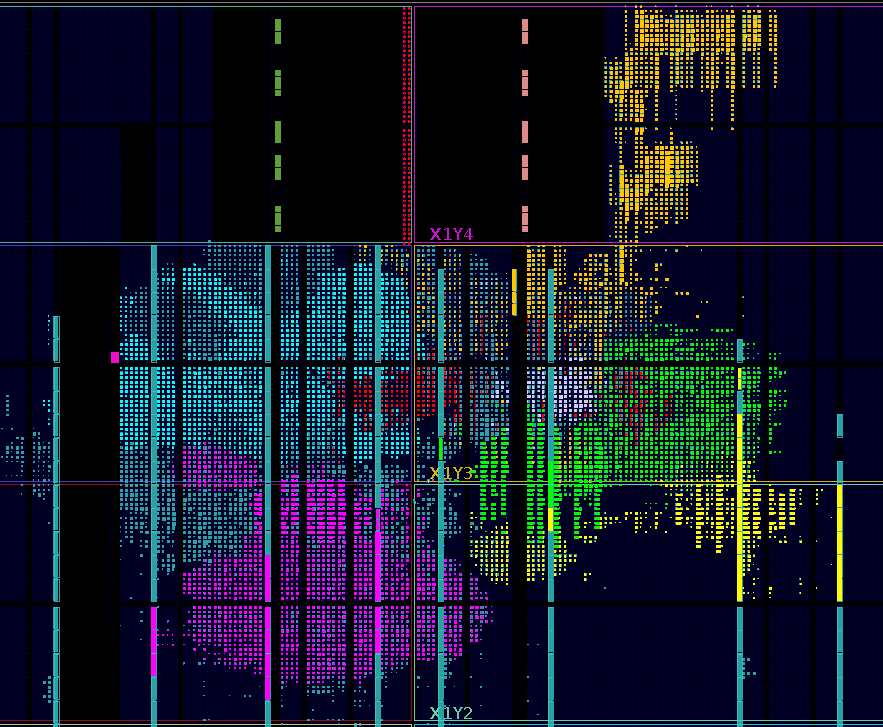
\includegraphics[width=0.5\linewidth]{colorful-new.png}
   \end{figure}
   
   \vspace{0.5 cm}
  
    \vspace{.5 cm}
    陈晟祺\\
    harry-chen@outlook.com\\
    \vspace{.5 cm}
    周聿浩\\
    miskcoo@gmail.com\\
    \vspace{.5 cm}
    刘晓义\\
    circuitcoder0@gmail.com\\
    \vspace{.5 cm}
    陈嘉杰\\
    jiegec@qq.com\\
  
    \vspace{1 cm}
    {\large \artdate}\\[3cm] 
  
  \vfill
  
\end{titlepage}

\tableofcontents

\chapter{概述}

\section{项目背景}

本项目的成果是在龙芯提供的FPGA实验平台上设计并实现基于 MIPS 32 的CPU,并使用实验板上的周边硬件,成为一个片上系统(SOC)。其能够支持标准MIPS 32 Rev 1指令集的一个较完整子集和 MIPS 32 Rev 2指令集的部分功能,能够运行功能、性能测试,并能够运行 u-boot 引导器、uCore 操作系统、Linux 操作系统等。

%在此之外,我们还完成了与编译原理的联合实验,能够运行 decaf 语言编写的程序。

\section{项目概览}

本项目计划设计和实现的部分主要包括:CPU、SoC设计、Bootloader、系统软件移植、自动化测试。项目使用的硬件语言为 SystemVerilog 2005。下面为各个部分的概览。

\subsection{CPU}

CPU 的设计包含指令集、流水线结构(微架构)、内存管理单元、异常处理机制、协处理器以及其他增强功能。

\begin{description}

    \item[指令集] 本项目的CPU实现的指令是 MIPS 32 Rev 1 指令集的一个较完整子集,包括了所有的算术逻辑指令、控制流指令和大部分特权指令(不包括与缓存有关的),覆盖了大赛要求需要的所有57条指令。MIPS 32 Rev 2 中的部分指令(如 CP0 中的 ebase 寄存器)由于被操作系统需要,也包含在实现中。
    \item[流水线结构] 本项目实现了具有\textbf{10段动态流水线}结构的\textbf{超标量(双发射)}处理器:根据流水线上处理指令的不同,以及当前指令与之前指令的数据/访存相关的不同,流水线各个阶段的操作也将不同。大致来说,流水线的各个阶段可以分为取指、译码、发射、执行、访存/延迟执行和写回。其中取指和访存各有3个阶段,发射有2个阶段。由于访存延迟过长,访存相关的暂停对性能影响较大,我们允许某些指令的执行延迟到访存阶段,即允许在译码阶段操作数未准备好的时候就发射指令,在其后操作数准备好时再执行。为了更好地支持超标量,我们的取指单元较为独立,获取的指令会放入指令FIFO,同时其有一个分支预测器。取指单元在分支预测成功的情况下保证生成的指令流就是执行所需的指令流,这处理了延迟槽等机制。取指单元一个周期至多会放入FIFO三条指令。
    \item[内存管理单元] 本项目实现了内存管理单元(MMU)以进行从虚拟地址到物理地址的映射,本项目的内存划分遵循 MIPS 32 标准,将使用转换检测缓冲区(TLB)以加速页表的查询,并对所有外设实现内存映射IO(MMIO)。
    \item[异常处理机制] 本项目完整支持 MIPS 32 Rev 1的异常和中断机制,正确处理同步和异步异常,支持硬件和软件中断,并实现精确异常。
    \item[协处理器] 本项目实现了 MIPS 32 Rev 1中为CP0处理器规定的几乎所有指令和寄存器,以正确运行操作系统。
    \item[缓存系统] 本项目实现了指令和数据缓存以及 MIPS 32 Rev 1 中要求的缓存控制指令,加快取指和访存。
    \item[增强功能] 本项目实现了一种可扩展的专用计算模块,它可以完成各类特殊的计算需求,例如密码学算法中的AES、SHA、MD5等。各个不同的计算单元通过统一的接口同CPU连接,计算单元通过其自身的寄存器与CPU交互。各类计算单元仅需要提供一个读写其自身寄存器的接口就可以直接接入CPU,具体和该模块的交互由软件通过MFC2和MTC2来完成。

\end{description}

\subsection{SoC设计}

为了验证 CPU 的设计,并且使用实验箱上提供的硬件进行更多的功能演示,我们以 NonTrivialMIPS CPU 为核心搭建了一个 SoC (System-on-Chip),具有以下模块:

\begin{description}

    \item[CPU] NonTrivialMIPS CPU (包含 Cache)
    \item[DRAM支持] 使用板载 DDR3 SDRAM 作为主存
    \item[额外存储] 板载 128KB BootROM 和 64KB RAM,用于初级引导程序
    \item[Flash读写] 支持软件通过 SPI 协议读取 FPGA 配置 Flash、读写扩展 Flash
    \item[串口] 16550 兼容的串口控制器,可调节波特率
    \item[以太网] 使用 Xilinx IP 构建的以太网控制器,实现 100Mbps 通信
    \item[GPIO] 使用龙芯 confreg 组件,软件控制 LED、数码管,读取开关、按键等状态
    \item[图像输出] 实现标准的 VGA Framebuffer,并实现了DMA 硬件加速绘制;支持使用外置 NT35510 LCD 绘制图像
    \item[PS/2] 支持 PS/2 键盘/鼠标输入
    \item[USB] 使用板载 USB PHY 提供 USB 2.0 Full Speed 控制器支持,支持人体工程学设备(键鼠)、大容量存储(U盘)等不同类型的设备
\end{description}

\subsection{Bootloader}

Bootloader用于引导操作系统,本项目中运行的 Bootloader分两个阶段,分别是自行编写的 TrivialBootloader 和移植的 U-Boot。前者是被固化在Bootrom中的程序,使用 C++ 边下,需要支持从Flash、SRAM、串口等多途径启动,提供任意地址转储等功能,负责基本的异常处理,并支持内存和外设的检查。而 U-Boot 是被TrivialBootloader加载的较复杂的引导程序,支持网络启动、Flash 启动、性能测试等高级功能,需要对源代码进行平台相关移植。


\subsection{操作系统移植}

我们在 SoC 上成功运行了 \texttt{uCore-thumips} 操作系统,并通过了其中的一系列测试。同时,我们将最新的 \texttt{Linux 5.2.8} 操作系统移植到实验板上,并成功运行;其能够使用 SoC 上的所有外设,包括串口、以太网、USB、图形输出等。我们在 Linux 上成功运行了大量用户态程序,包括 GNU 命令行工具、Xorg Server、Python 解释器等。

% 我们在板上系统上成功运行了 \texttt{uCore-thumips} 操作系统,包括进行一些平台相关的改动,以及正确实现CPU的各项功能(尤其是MMU相关模块)、正确与外设进行通信。为了演示本项目的成果,我们还在操作系统上编写了数个用户态程序,并移植 USB 键盘驱动到内核。同时,我们也为 decaf 编译器后端编写了对应的链接库,以使其编译出的 MIPS 汇编能够正常在我们的平台上运行,并支持输入、输出等功能。

% \todo

\subsection{自动化测试与部署}

本项目还使用了基于GitLab CI的自动化综合、测试、部署系统,包括以下的功能:

\begin{itemize}

    \item 项目需求、设计等文档的自动编译
    \item 基于事先撰写的 testbench 自动对CPU、外设和整个板上系统运行RTL仿真
    \item 自动调用 Vivado 生成 Bitstream 文件,并缓存可复用的中间结果
    \item 所有相应软件的自动编译,使用 QEMU 对操作系统进行测试
    \item 使用在线实验平台 SDK,在真实环境中运行性能、功能测试和操作系统,并提取数据进行分析和报告

\end{itemize}

\section{名词解释}

表\ref{table:abbreviation_definition}中是本项目中可能用到的一些名词缩写及它们的解释,以后本项目相关的文档中将不加解释地使用这些缩写。

\begin{table}[!htbp]
    \centering
    \caption{名词缩写和解释}
    \label{table:abbreviation_definition}
    
    \begin{tabular}{|l|l|l|}
    \hline
    \multicolumn{1}{|c|}{\textbf{缩写}} & \multicolumn{1}{c|}{\textbf{全称}}                   & \multicolumn{1}{c|}{\textbf{含义}} \\ \hline
    MIPS                              & Microprocessor without Interlocked Pipeline Stages & 无内部互锁流水级的微处理器                    \\ \hline
    CPU                               & Central Processing Unit                            & 中央处理器                            \\ \hline
    FPU                               & Floating Point Unit                                & 浮点处理器                            \\ \hline
    CP0/1                             & Co-Processor 0/1                                   & 协处理器 0/1                         \\ \hline
    ALU                               & Arithmetic Logic Unit                              & 算术逻辑单元                           \\ \hline
    MMU                               & Memory Management Unit                             & 内存管理单元                           \\ \hline
    TLB                               & Translation Lookaside Buffer                       & 旁路快表缓冲                           \\ \hline
    PA/VA                             & Physical/Virtual Address                           & 物理/虚拟地址                          \\ \hline
    ROM                               & Read Only Memory                                   & 只读存储器                            \\ \hline
    (D)RAM                            & (Dynamic) Random Access Memory                     & (动态)随机访问存储器                      \\ \hline
    UART                              & Universal Asynchronous Receiver-Transmitter        & 通用异步接收器-发射器                      \\ \hline
    GPIO                              & General-Purpose Input/Output                       & 通用目的输入/输出                        \\ \hline
    MMIO                              & Memory Mapped Input/Output                         & 内存映射输入/输出                        \\ \hline
    USB                               & Universal Serial Bus                               & 通用串行总线                        \\ \hline
    SOC                               & System On a Chip                                   & 片上系统                             \\ \hline
    \end{tabular}
\end{table}

\section{开发平台}

\subsection{硬件平台}

本项目使用的硬件平台为龙芯FPGA实验箱,其主要部件为Xilinx的Artix 7系列FPGA,型号为xc7a200t,包含外部器件:

\begin{description}
    \item[DRAM] 128MB DDR3 SDRAM 
    \item[NOR Flash (CFG)] 16MB
    \item[NOR Flash (SPI)] 32MB
    \item[VGA 接口] RGB输出,各 4 bit 
    \item[以太网接口] DM9161 100Mbps Ethernet PHY 
    \item[其他接口] 标准 RS232 串口、PS/2 接口、USB PHY
    \item[显示屏] NT35510 LCD,分辨率 800 $\times$ 480
    \item[GPIO] 数码管 $\times$  8,LED $\times$  26,拨码开关 $\times$ 8,按键 $\times$ 19
\end{description}

\subsection{软件平台}
\label{section:software_platform}

本项目使用 GitLab-CI 进行自动化集成和测试,借助Docker保证运行结果可复现。

\begin{description}
    \item[开发IDE] Xilinx Vivado 2018.3 Web HL Edition
    \item[CI系统] Ubuntu 18.04.1
    \item[编译器套件] cross-mipsel-linux-gnu-binutils 2.32-1, cross-mipsel-linux-gnu-gcc 9.1.0-1 (AUR)
\end{description}

\section{参考资料}

本项目的设计、开发过程需要参考包括且不限于下面列出的书籍、文献和资料:
\begin{itemize}
    \item \textit{计算机组成与设计: 硬件/软件接口.} David A.Patterson
    \item \textit{See MIPS Run Linux.} Dominic Sweetman
    \item \textit{自己动手写CPU.} 雷思磊
    \item \textit{MIPS® Architecture For Programmers I, II, III.} Imagination Technologies LTD.
    \item \textit{Vivado使用误区与进阶.} Ally Zhou
    \item \textit{NaiveMIPS 设计文档.} 张宇翔,王邈,刘家昌
    \item \textit{32-bits MIPS CPU 设计文档.} 谢磊,李北辰
    \item \textit{各外设使用手册.} 相关厂商
\end{itemize}


\chapter{CPU}

\section{流水线结构}

\subsection{总体架构}

CPU采用双发射顺序执行,共有10级流水。整体的流水线结构如图 \ref{fig:cpu-pipeline} 所示。其中为了能够得到较高的频率,指令和数据Cache均采用3级流水。为了解决访存周期过长而导致的访存暂停过多,我们动态地判断指令的执行时间,允许指令在操作数没有准备好时就发射,并且在操作数准备好时再执行。流水线各个阶段的功能会根据指令类型和数据相关情况动态变化。

各个阶段的功能大致如下:
\begin{itemize}
    \item \textbf{取指1} 计算当前PC,发送请求给指令Cache。
    \item \textbf{取指2} 指令Cache读取数据。
    \item \textbf{取指3} 对指令进行简单译码,进行简单的分支解析,将指令包放入FIFO。
    \item \textbf{译码/发射}\, 从FIFO获取指令包,进行译码并且决定是否发射。
    \item \textbf{读操作数}\, 从寄存器堆以及数据旁路读取操作数。
    \item \textbf{执行}\, 执行指令。读取存储指令的数据。
    \item \textbf{访存1/延迟读操作数}\,  向数据Cache发送访存请求。同时处理异常,对于延迟执行的指令进行操作数读取。
    \item \textbf{访存2/延迟执行}\, 数据Cache计算数据。延迟执行的指令在此时执行。
    \item \textbf{访存3}\, 读取访存结果。
    \item \textbf{写回}\, 写回数据到寄存器堆。
\end{itemize}

\begin{landscape}
\begin{figure}[htbp]
	\centering
	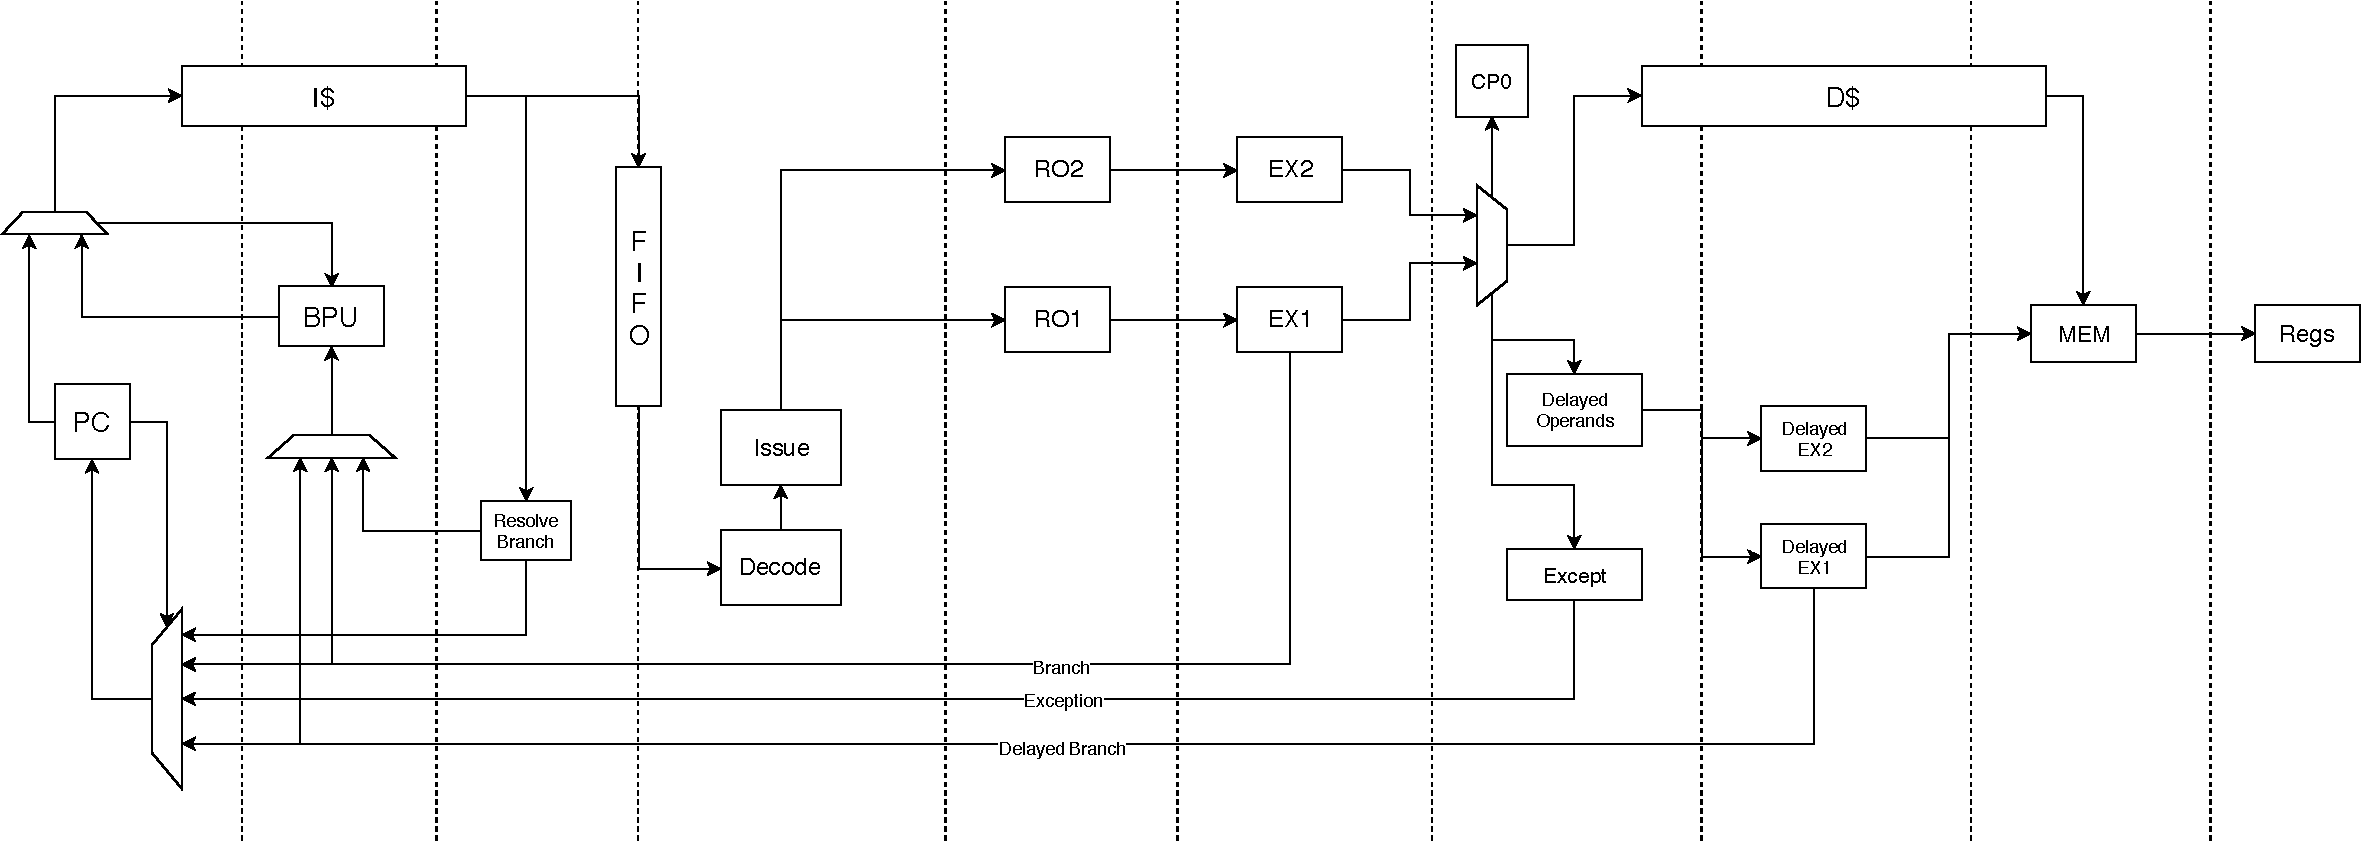
\includegraphics[width=\linewidth]{cpu-design.pdf}
	\caption{CPU流水线结构}
	\label{fig:cpu-pipeline}
\end{figure}
\end{landscape}

\subsection{取指阶段}
取指阶段共有3级流水,最后得到的指令会放入指令FIFO。在此3阶段中同时会进行分支预测,同时能够保证在分支命中的情况下放入FIFO的指令流就是所需要执行的指令流。分支预测失败会刷新指令FIFO,该信息由执行单元生成。

分支预测采用传统的2比特分支预测,BTB和BHT采用BRAM实现,延迟为一个周期。

取指的第一个阶段,会计算取指的地址并且发送给Cache,同时计算下一个PC的值。

取指的第二个阶段,会对下一个阶段需要放入FIFO的指令包的一部分内容进行计算。

取指的第三个阶段,会对得到的指令进行简单的译码,判断是否为分支同时反馈给分支预测和PC生成器。如果将非分支指令预测为分支,那么及时进行流水线刷新。此阶段还会将指令包放入指令FIFO,至多会有3条指令被放入(即第二条指令是分支,并且延迟槽和分支在同一个Cache行中)。

当前周期所需要取指的地址通过当前PC和BTB/BHT得到的分支信息得到,下一个周期的PC受到当前PC,分支预测信息,指令FIFO是否满,异常请求和执行阶段所解析的分支信息控制。如果指令FIFO满则会丢弃当前数据并且重新在对应为止取指。

为了支持多发射流水线,指令Cache要求地址按照8字节对齐,每次会返回64位的数据,另外如果随后的64位数据仍然在Cache行内,也会将其返回,这是为了更快地处理延迟槽。由于MIPS具有延迟槽机制,我们在分支预测跳转之后还需要将延迟槽也放入指令FIFO。为了尽量获取更多的指令,如果指令Cache返回的64或者128位数据中有延迟槽,那么当前就可以直接取分支目标的指令,否则需要取延迟槽指令。

\subsection{译码和发射阶段}
译码和发射均在流水线的第4个阶段。译码器会从指令FIFO中获取对应信息,并且进行译码。

发射阶段较为复杂,其共分为如下几种情况
\begin{enumerate}
    \item 由于我们的流水线设计中仅有一个乘法器和除法器,乘除指令一个周期内最多只能发射一条。另外,为了设计简便,CP0相关指令一个周期内也最多只能发射一条。除此之外,由于只有一个访存单元,访存指令在一个周期最多也只发射一条。
    \item 如果一个发射包内两条指令存在数据相关,那么只发射第一条指令。
    \item 分支指令必须和延迟槽一起发射,如果延迟槽没有取到则需要暂停,如果分支指令是发射包第二条指令则不能发射。
\end{enumerate}

由于访存结果在流水线第9个阶段才能得到,如果在译码阶段直接读操作数则访存相关需要3个周期的暂停。为了更好地处理访存相关,我们进行部分指令的延迟执行。具体来说,如果指令在译码阶段后不会产生异常(例如AND,XOR,ADDU等),我们可以将这类指令的操作数读取延迟到访存的第一阶段,执行延迟到访存的第二阶段。这样访存相关的暂停最好可以缩短到一个周期。更进一步,我们还可以将分支指令也推迟到这个阶段。但是由于分支有可能预测失败,我们需要能够撤销其后的指令。幸运的是,访存请求的提交和异常的触发都是在访存第一阶段,而分支指令的解析是在访存第二阶段,并且其延迟槽不会有异常。这样恰好可以在解析到分支预测失败时刷新流水线,使得其后的指令不会改变处理器状态。

当然,如果指令不能延迟执行,那么仍然需要暂停到操作数均可用为止。此时的访存相关还要考虑正在延迟执行的指令而不仅仅是访存指令。

总的来说,在发射阶段需要暂停的情况大致如下:
\begin{enumerate}
    \item 指令无法延迟执行,并且操作数没有准备好。这包含访存指令数据没有准备好,以及延迟执行的指令结果没有准备好。
    \item 指令可以延迟执行,但是在执行阶段有访存指令。这是真正的无法消除的访存相关。
    \item 分支指令但是延迟槽还不在FIFO中。
    \item 执行阶段正在执行特权指令。这是由于CP0的设计原因。
    \item 流水线上存在非MFC0和MTC0的特权指令,这是为了解决可能的CP0冒险。
\end{enumerate}

\subsection{读操作数阶段}
指令所需要的两个操作数在第5个阶段从寄存器堆和数据旁路读取。对于延迟执行的指令,此时读取的操作数可能是无效的,会在之后再次读取。对于存储指令,存储的数据可能是无效的,会在执行阶段再次读取。

\subsection{执行阶段}
执行阶段是流水线的第6个阶段。此阶段会生成指令的结果,同时计算异常请求,计算访存地址。

对于内存写指令(如SW、SC等)会在此阶段读取需要写的数据。对于多周期指令,在计算完前会生成一个暂停信号。流水线仅有一个乘法和除法单元。

\subsection{访存阶段}
访存阶段是流水线的第7, 8, 9阶段,在第7阶段将访存请求发送给数据Cache,在第9个阶段可以得到访存结果。

该阶段和延迟执行阶段是重叠的。

\subsection{延迟执行阶段}
大部分指令都是在译码阶段读取操作数,在执行阶段计算结果。如果指令之间存在访存相关,并且指令是分支或者不会在执行阶段出现异常,那么其可以在流水线第7阶段读取操作数,其后一个阶段计算结果。如果是分支指令则会生成分支结果反馈给分支预测器。

该阶段和访存阶段是重叠的。

\subsection{写回阶段}
此阶段写回寄存器请求,是流水线的最后一个阶段。
\section{指令集}
下方按照功能划分列举了CPU所支持的MIPS指令,各条指令的具体编码以及功能在MIPS文档中有详细的描述。
\begin{itemize}
	\item \textbf{自陷指令} TGE, TEGU, TLT, TLTU, TEQ, TNE, TGEI, TGEIU, TLTI, TLTIU, TEQI, TNEI
	\item \textbf{分支指令} BLTZ, BGEZ, BLTZAL, BGEZAL, BEQ, BNE, BLEZ, BGTZ, JR, JALR, J, JAL
	\item \textbf{逻辑指令} AND, OR, XOR, ANDI, ORI, XORI, NOR, SLL, SRL, SRA, SLLV, SRLV, SRAV
	\item \textbf{算术指令} ADD, ADDU, SUB, SUBU, ADDI, ADDIU, MUL, MULT, MULTU, DIV, DIVU, MADD, MADDU, MSUB, MSUBU, CLO, CLZ
	\item \textbf{访存指令} SB, SH, SW, SWL, SWR, LB, LH, LWL, LWR, LW, LBU, LHU, LL, SC
	\item \textbf{特权指令} CACHE, SYSCALL, BREAK, TLBR, TLBWI, TLBWR, TLBP, ERET, MTC0, MFC0
	\item \textbf{条件移动指令} SLT, SLTU, SLTI, SLTIU, MOVN, MOVZ
	\item \textbf{无条件移动指令} LUI, SLT, SLTU, MFHI, MFLO, MTHI, MTLO 
\end{itemize}

\section{协处理器0}
CP0是MIPS规范中必要的一个协处理器,它提供了操作系统所必须的功能抽象,例如异常处理、内存管理和资源访问控制等。

在CP0中有多个32位寄存器,各个寄存器均通过MTC0和MFC0读写。另外,诸如TLBWI、TLBWR和TLBP等特权指令还有异常的发生也有可能会影响其值。

表\ref{table:required_cp0_registers}中列出了必须实现的CP0寄存器。

\begin{table}[!htbp]
    \centering
    \caption{必要的CP0寄存器}
    \label{table:required_cp0_registers}
    \begin{tabular}{|r|l|l|}
    \hline
    \textbf{编号} & \textbf{名称} & \textbf{功能}  \\ \hline
	8 & BadVAddr & 最近发生的与地址相关的异常所对应的地址 \\ \hline
	9 & Count & 计数器 \\ \hline
	11 & Compare & 计时中断控制器 \\ \hline
	12 & Status & 处理器状态及控制 \\ \hline
	13 & Cause & 上一次异常的原因 \\ \hline
	14 & EPC & 上一次异常发生的地址 \\ \hline
	15 & PRId & 处理器版本和标识符 \\ \hline
	16 & Config0 & 处理器配置 \\ \hline
	30 & ErrorEPC & 上一次异常发生的地址 \\ \hline
    \end{tabular}
\end{table}

为了实现TLB MMU的功能,还需要表\ref{table:mmu_cp0_registers}中所列出的寄存器。

\begin{table}[!htbp]
    \centering
    \caption{MMU所需要的CP0寄存器}
    \label{table:mmu_cp0_registers}
    \begin{tabular}{|r|l|l|}
    \hline
    \textbf{编号} & \textbf{名称} & \textbf{功能}  \\ \hline
	0 & Index & TLB数组的索引 \\ \hline
	1 & Random & 随机数 \\ \hline
	2 & EntryLo0 & TLB项的低位 \\ \hline
	3 & EntryLo1 & TLB项的低位 \\ \hline
	4 & Context & 指向内存中页表入口的指针 \\ \hline
	5 & PageMask & 控制TLB的虚拟页大小 \\ \hline
	6 & Wired & 控制TLB中固定的页数 \\ \hline
	10 & EntryHi & TLB项的高位 \\ \hline
    \end{tabular}
\end{table}

同时,为了支持自定义异常向量,还需要额外实现一个MIPS 32 Rev 2 中的 EBase寄存器。

\section{中断和异常}
\subsection{中断}
MIPS的中断一共有8个,从0开始编号。其中0号中断和1号中断是软件中断,由软件设置Cause寄存器中的对应位来触发。其余6个中断为硬件中断,由外部硬件触发。在实现中,由Count/Compare寄存器组合而成的定时中断的中断号为7。

如果该中断满足触发条件则会触发异常并且进入中断处理程序。中断的触发要求如下条件全部满足:
\begin{enumerate}
	\item \texttt{Status}寄存器中对应的中断被打开;
	\item 全局中断使能,即\texttt{Status.IE}为1;
	\item 当前不在异常处理程序中,即\texttt{Status.EXL}和\texttt{Status.ERL}为0。
\end{enumerate}

\subsection{异常}
MIPS的异常是“精确异常”,也就是在异常发生前的指令都会执行完毕,异常发生之后的指令不会继续执行。在异常发生时,CPU会跳转到对应的异常向量处执行异常处理代码并设置CP0中对应的寄存器记录异常的原因和一些额外的信息,同时还会进入Kernel Mode。处理异常代码的异常向量由“基地址+偏移”来决定,偏移是根据异常来确定的,基地址是由CP0的EBase寄存器决定。

在我们的实现中,在流水的各个阶段产生了异常,不会马上触发,而是被记录下来,顺着流水直到MEM阶段完成后再进行触发。同时,还会考虑双发射两条流水线,优先触发第一条流水线的异常。特别地,异常返回指令ERET被实现为一种特殊的异常,保留到MEM阶段触发。

需要支持的异常在表\ref{table:main-exception}中列出。

\begin{table}[htbp]
	\centering
	\caption{主要支持的异常}
	\label{table:main-exception}
	\begin{tabular}{|c|c|c|c|} \hline
		\textbf{异常简称} & \textbf{异常说明} & 	\textbf{异常简称} & \textbf{异常说明} \\ \hline
		Int & 中断   & Sys & 系统调用             \\ \hline
		Mod & TLB修改异常 & 	Bp & 断点  \\ \hline
		TLBL & TLB Load异常 & 	RI & 保留指令 \\ \hline
		TLBS & TLB Store异常 & 	CpU & 协处理器不可用 \\ \hline
		AdEL & 地址Load异常 & Ov & 算术溢出\\ \hline
		AdES & 地址Store异常 & 	Tr & 自陷异常 \\ \hline
	\end{tabular}
\end{table}
\section{内存管理}
MIPS为操作系统的内存管理提供了较为简单的支持,虚拟地址通过MMU转换为物理地址。MIPS标准对虚拟地址和物理地址的映射如表\ref{tab:virtual-address-space}所示。

\begin{table}[htbp]
	\centering
	\caption{虚拟地址空间}
	\label{tab:virtual-address-space}
	\begin{tabular}{|c|c|c|c|} \hline
		\textbf{段} & \textbf{虚拟地址} & \textbf{权限} & \textbf{物理地址} \\ \hline
		kseg3/ksseg & \texttt{0xC000000-0xFFFFFFFF} & Kernel & 由TLB转换 \\ \hline
		kseg1 & \texttt{0xA0000000-0xBFFFFFFF} & Kernel & \texttt{0x00000000-0x1FFFFFFF} \\ \hline
		kseg0 & \texttt{0x80000000-0x9FFFFFFF} & Kernel & \texttt{0x00000000-0x1FFFFFFF} \\ \hline
		useg &  \texttt{0x00000000-0x7FFFFFFF} & User & 由TLB转换 \\ \hline
	\end{tabular}
\end{table}

具体的地址转换由TLB来完成,TLB可以认为是在CPU内部的地址转换表的高速缓存。具体的内容需要由操作系统来进行填充。如果在TLB中没有找到对应虚拟地址则会触发一个TLB miss异常,操作系统对该异常处理,并且将对应转换表填入TLB中的某一项来完成对地址的转换。我们一共实现了16个TLB项。

\section{增强功能}
\label{sec:enhancement}

我们实现了一种可扩展的专用计算模块,它可以完成各类特殊的计算需求,例如密码学算法中的AES、SHA、MD5等。各个不同的计算单元通过统一的接口同CPU连接,计算单元通过其自身的寄存器与CPU交互。各类计算单元仅需要提供一个读写其自身寄存器的接口就可以直接接入CPU,具体和该模块的交互由软件通过MFC2和MTC2来完成。

CPU通过MTC2和MFC2两条指令来访问各个功能部件,其指令格式如图 \ref{fig:cp2-instruction} 所示。

\begin{figure}[htbp]
    \centering
    \begin{bytefield}[endianness=big]{32}
    \bitheader{0-31} \\
    \bitbox{6}{010010} & \bitbox{5}{CF} & \bitbox{5}{rt} & \bitbox{1}{E} & \bitbox{7}{C} & \bitbox{8}{R}
    \end{bytefield}
    \caption{CPU扩展指令(CP2协处理器)格式}
    \label{fig:cp2-instruction}
\end{figure}

MTC2用于将CPU寄存器的值移入计算单元的寄存器中,MFC2用于读取计算单元寄存器值。MTC2对应的CF为00100,MFC2对应的CF为00000。其中rt表示CPU寄存器的编号,E表示传输的数据的端序是否与CPU端序不同。C表示功能部件的ID,R表示计算单元的寄存器编号。

作为示例,我们利用开源的AES模块\footnote{\url{https://github.com/secworks/aes}}实现了AES128和AES256的硬件计算单元,其有8个密钥寄存器,4个输入寄存器,4个输出寄存器,它们分别存放计算AES所需的数据。同时,还有一个控制寄存器和一个状态寄存器。控制寄存器用于告诉计算模块数据是否准备好,是否开始计算以及密钥长度等信息。状态寄存器用于获取当前模块是否可用以及计算是否完成。

\section{缓存设计}
CPU 提供指令缓存和数据缓存,分别处理取指和访存请求,并实现了最小化的 CACHE 控制指令。所有的缓存均为虚拟索引物理标签(VIPT)。
\subsection{指令缓存}
指令缓存提供了取指支持,大小和相连度可配置,采用三级流水,其第一个流水段接受请求,并且读取对应的TAG和数据。第二个流水段判断是否命中,第三个流水段给出数据。如果不命中,在第三流水段通过 AXI 和外设通信读入。由于采用双发射执行,指令缓存每次读取返回两条指令,并且如果下一条指令也在缓存中的话,也一起取出。

MIPS 要求 CACHE 控制指令必须实现清除特定地址或者索引位置的数据缓存。由于清除每一路对应索引位置的缓存包含了清除特定地址,所以我们将这两个请求都实现为清除了特定索引位置的所有缓存。

\subsection{数据缓存}
数据缓存提供了访存支持,包括经过缓存和不经过缓存两个类型的访存。根据 MIPS 标准要求,对于不同段的访存,数据缓存行为不同。

\begin{itemize}
	\item \textbf{kseg3/ksseg} 按 TLB 判断是否经过缓存
	\item \textbf{kseg1} 不经过缓存
	\item \textbf{kseg0} 可以由 CP0 $\mathrm{Config_{K0}}$ 寄存器控制,MIPS 标准中这一行为的实现可选
    \item \textbf{useg} 按 TLB 判断是否经过缓存
\end{itemize}

在 NonTrivialMIPS CPU 中,数据缓存使用延迟写回的实现,写失效时进行写分配,包含写合并操作,大小和相连度可配置。当访存位置的数据在缓存或者写回 FIFO 中时,可以保证在一个周期内完成读写,避免流水线暂停。使用延迟写回可以同时利用 AXI 总线上的读写通道。

\begin{figure}[htbp]
	\centering
	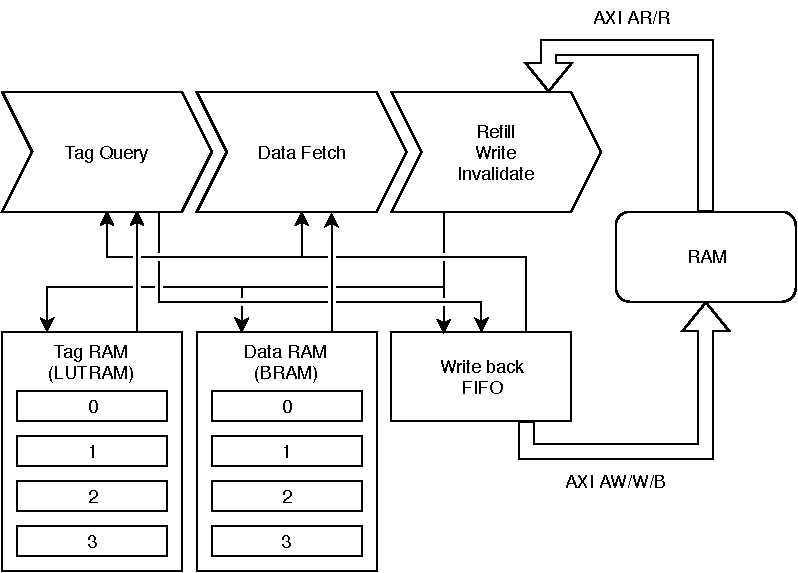
\includegraphics[width=\linewidth]{dcache.pdf}
	\caption{数据缓存结构}
	\label{fig:dcache-structure}
\end{figure}

数据缓存共包含三级流水,结构如图 \ref{fig:dcache-structure} 所示。每一路数据缓存中包含两个 RAM 存储,分别包含每个索引位置的标签和数据。为了能够快速读取,标签存储使用 Xilinx Parameterized Macros 生成的 LUT RAM,可以实现在当前周期读出数据。数据 RAM 使用 Xilinx Parameterized Macros 生成的 Block RAM。

数据缓存还包含一个 FIFO,作为延迟写回的队列。为了实现写合并,FIFO 提供一个额外的随机访问接口,可以使用 FIFO 中某一行的地址完成对于 FIFO 的随机读写。

对于读请求,数据缓存的工作流程如下。
\begin{itemize}
  \item \textbf{第一阶段} 完成对于标签的查询,写回 FIFO 的查询,计算得到缓存命中。
  \item \textbf{第二阶段} 从数据 RAM 中取得对应索引位置的数据,计算读出的数据。
  \item \textbf{第三阶段} 给出数据。如果缓存缺失,通过 AXI 和外设通信,更新缓存,并将覆写位置的脏数据送入 FIFO 中。
\end{itemize}

对于写请求,数据缓存的工作流程如下。
\begin{itemize}
  \item \textbf{第一阶段} 完成对于标签的查询,计算得到缓存命中,完成对于 FIFO 中的写合并操作。
  \item \textbf{第二阶段} 得到数据 RAM 对应索引位置的数据,根据 byteenable 计算得出需要写入数据 RAM 的数据。
  \item \textbf{第三阶段} 完成对标签、数据 RAM 的写入。如果缓存缺失,则进行写分配,并将覆写位置的脏数据送入 FIFO 中。
\end{itemize}

MIPS 要求 CACHE 控制指令必须实现清除、写回特定地址或者索引位置的数据缓存。由于清除也包含写回操作,所以和指令缓存相同,我们实现了清除每一路缓存的特定索引位置,并等待脏数据写回完成。


\section{外部接口}

CPU 整体的结构如图 \ref{fig:cpu-interface} 所示,NonTrivialMIPS CPU 本身暴露三个 AXI 4 Master 接口,分别进行指令读取、数据存取和不过缓存的数据存取。Cache 控制器与 CPU 之间使用自定义的总线信号进行握手和数据传输,以避免在内部使用 AXI 协议带来的不必要延时;而对外,则将必要的访存转换为符合 AXI 规范的信号,与 SoC 进行交互。

由于预赛 \texttt{myCPU} 目录中的 CPU 顶层模块对外只允许暴露一个 AXI 3 Master 接口,我们使用 Xilinx 的 AXI Crossbar IP 将其转换为三个 AXI 4 Slave 接口以适应 CPU 的需要。为了不使得指令预取阻塞访存,crossbar 上的仲裁顺序为 Passthrough > Data Cache > Instruction Cache。在CPU 直接连接到我们设计的 SoC 时,则不使用这一 crossbar,而是将三个 AXI 4 Master 接口直接连接到 Interconnect 上。

\begin{figure}[htbp]
	\centering
	\includegraphics[width=\linewidth]{cpu-interface.pdf}
	\caption{CPU 整体接口架构}
	\label{fig:cpu-interface}
\end{figure}

	

\chapter{SoC 设计}

\section{概况}

为了更好地利用实验板提供的硬件资源,对 NonTrivialMIPS 进行功能演示,我们搭建了一个较为完整的 SoC,能够在大赛提供的实验箱上运行。

\subsection{SoC结构}

\begin{figure}[htbp]
    \centering
    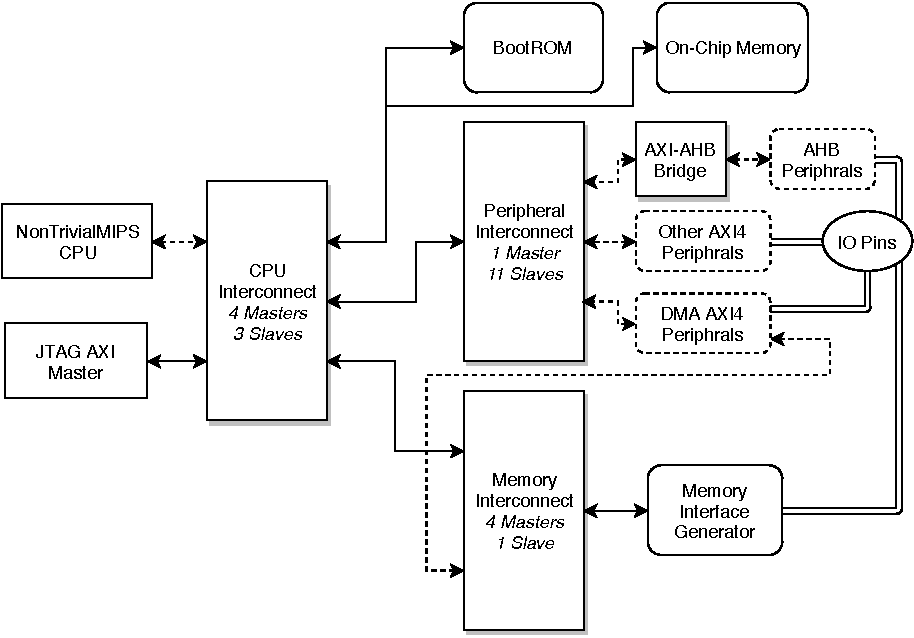
\includegraphics[width=\linewidth]{soc-structure.pdf}
    \caption{SoC结构}
    \label{fig:soc-structure}
\end{figure}

SoC由 Vivao 的 Block Design 设计功能组件,项目文件为 \texttt{vivado/NonTrivialMIPS.xpr},总体结构如图 \ref{fig:soc-structure} 所示。其中各个组件之间均使用标准的 AXI4 总线协议进行连接,并使用了多个 AXI Interconnect。图中无阴影的矩形表示 AXI Master,带阴影的矩形表示 AXI 总线互联(Interconnect)或适配器(Bridge),圆角矩形表示外设。图中的所有实线表示其为具体设备(及其连接关系),虚线表示由多个具体设备构成的一类设备(及其连接关系),双线表示到 FPGA 片外的连接。

我们将 NonTrivialMIPS CPU 的三个 AXI 接口(指令 Cache、数据 Cache、无 Cache 直通)直接连接到 CPU 互联模块上,不再需要预赛时 CPU 内部的互联模块。这一互联模块上还连接了 Xilinx 提供的 JTAG AXI Master IP,可以绕过 CPU 直接与设备进行通信,方便进行调试。这一互联模块直接连接了 BootROM 与片上 RAM(OCM) 两个使用 FPGA 的 Block RAM 资源生成的存储,以及外设互联、内存互联模块。这一设计使得 TrivialBootloader 等程序可以无需运行在内存中,而是在 OCM 中分配堆栈资源。这样,它就可以在内存的任意位置加载操作系统,而不用担心自身代码或数据被覆盖;并且当系统发生不可逆转或者没有捕获的异常/错误时,其依旧可以获取系统控制权,输出必要的调试信息后安全地停止工作。

外设互联模块上连接了除 DDR 内存控制器外所有的外设,其中由于部分外设使用 AHB 协议,我们额外连接了一个 AXI 到 AHB 协议的转换桥。

内存互联模块只有一个从设备,即 Xilinx 的 Mmemory Generator Interface IP 模块。在正确配置后,其能自动对板载的 DDR3 SDRAM 进行训练等操作,并将自己暴露为一片连续的存储空间供用户使用,隐藏了所有实现细节。除 CPU 互联模块外,内存互联的主设备还包含所有有 DMA 需求的外设,包括 VGA 控制器、FrameBuffer 读写控制器等。这样的连接能够让硬件在空闲时直接对内存进行读写,而无需 CPU 干预,大大加速了图形渲染、内存修改等过程。

\subsection{地址分配}

表 \ref{table:address_allocation} 列举了各个设备的物理地址空间分配,其对于总线上的所有 Master 设备都是一致的。

\begin{table}[!htbp]
    \centering
    \caption{外设物理地址分配}
    \label{table:address_allocation}
    \begin{tabular}{|c|c|c|c|c|}
    \hline
    \textbf{名称} & \textbf{起始地址} & \textbf{结束地址} & \textbf{有效大小} & \textbf{类型} \\ \hline
    DDR 控制器        & 0x00000000    & 0x07FFFFFF    & 128 MB          & 存储          \\ \hline
    OCM 控制器       & 0x08000000    & 0x0800FFFF    & 64 KB          & 存储          \\ \hline
    CFG Flash 控制器(内存映射) & 0x1A000000    & 0x1AFFFFFF    & 16 MB          & 存储          \\ \hline
    以太网控制器    & 0x1C000000    & 0x1C00FFFF    & 64 KB      & 寄存器          \\ \hline
    VGA 控制器        & 0x1C010000    & 0x1C01FFFF    & 64 KB         & 寄存器         \\ \hline
    PS/2 控制器        & 0x1C020000    & 0x1C020FFF    & 4 KB         & 寄存器         \\ \hline
    LCD 控制器        & 0x1C030000    & 0x1C030FFF    & 4 KB         & 寄存器         \\ \hline
    SPI Flash 控制器        & 0x1C040000    & 0x1C040FFF    & 4 KB         & 寄存器         \\ \hline
    USB 控制器        & 0x1C050000    & 0x1C050FFF    & 4 KB         & 寄存器         \\ \hline
    Framebuffer Reader 控制器        & 0x1C060000    & 0x1C06FFFF    & 64 KB         & 寄存器         \\ \hline
    Framebuffer Writer 控制器        & 0x1C070000    & 0x1C07FFFF    & 64 KB         & 寄存器         \\ \hline
    外部中断控制器        & 0x1D000000    & 0x1D00FFFF    & 64 KB         & 寄存器         \\ \hline
    BootROM 控制器       & 0x1FC00000    & 0x1FC1FFFF    & 128 KB          & 存储          \\ \hline
    串口控制器       & 0x1FD02000    & 0x1FD03FFF    & 8 KB          & 寄存器          \\ \hline
    GPIO 控制器       & 0x1FF00000    & 0x1FF0FFFF    & 64 KB          & 寄存器          \\ \hline

    \end{tabular}
\end{table}

\subsection{中断连接}

一些外设需要通过中断告知 CPU 自身的状态而完成 IO 操作。MIPS 规范中 CPU 至多支持 5 个外部中断(编号为 2 到 6),并且 NonTrivialMIPS 只支持电平触发的中断。因此,我们使用了 Xilinx Interrupt Controller IP 来对类型不同或者超出数量限制的中断进行统一转换和管理。表 \ref{table:interrupt-connection} 描述了这些中断的连接关系。

\begin{table}[!htbp]
    \centering
    \caption{中断连接关系}
    \label{table:interrupt-connection}
    \begin{tabular}{|c|c|c|c|}
    \hline
    \textbf{名称} &  \textbf{中断类型} & \textbf{接收方} & \textbf{中断编号} \\ \hline
    串口控制器       & 高电平    & CPU     & 2          \\ \hline
    PS/2 控制器       & 高电平    & CPU     & 3          \\ \hline
    AXI 中断控制器       & 高电平    & CPU     & 6          \\ \hline
    以太网控制器       & 上升沿    & AXI中断控制器     & 0          \\ \hline
    SPI Flash 控制器       & 上升沿    & AXI中断控制器     & 1          \\ \hline
    CFG Flash 控制器       & 上升沿    & AXI中断控制器     & 2          \\ \hline
    USB 控制器       & 高电平    & AXI中断控制器     & 3          \\ \hline
    \end{tabular}
\end{table}

\section{硬件支持}

FPGA 板载了较多的物理接口和硬件资源,为了充分利用,达到较好的展示效果,我们均对它们进行了适配。

\subsection{串口控制器}

板载串口为 RS-232 接口,我们使用 Xilinx 提供的 AXI UART 16550 IP 实现了一个标准的 NS16550 UART 控制器。其支持比较完整的串口协议,包括可变波特率、流量控制和读写缓冲区。在软件使用串口前,需要首先对多个配置寄存器进行初始化,配置波特率、中断等不同的属性,方可正常与 PC 进行通信。串口控制器有一个中断,指示收到了数据,它被直接连接到 CPU 的第一个硬件中断上。

\subsection{USB 控制器}

实验箱上的 USB PHY 为 Microchip USB 3500 ,支持 Host/Device/OTG 三种模式下的 USB 2.0 协议。它提供的是 UTMI+ Level 3.0 的接口,我们从实验箱的原理图中找到了对应引脚在 FPGA 上的绑定,并添加到约束文件中。由于 USB 3500 仅实现了物理层的收发逻辑,我们以开源的 UltraEmbedded USB 1.1 Host Controller IP 为基础,进行了大量的修改以满足使用需求。具体工作将工作频率调整为 USB 2.0 Full Speed 指定的 60MHz、调整 IFS 逻辑、添加输出延迟约束等等。此外,我们也需要移植驱动到 U-Boot 和Linux 中,这将在下面的系统软件部分中详述。

\subsection{以太网控制器}USB

实验箱上提供了一个 10/100 Mbps 的以太网 PHY (物理接口),引出了以太网协议中规定的标准的 MII 和 MDIO 接口,用于数据传输和物理芯片配置。我们使用了 Xilinx 提供的 AXI Ethernet Lite IP 实现以太网控制器,在 U-Boot 和 Linux 中都有对应的驱动。这一控制器不支持 DMA,因此实际的数据传输无法达到 100 Mbps 全速工作。事实上,经过测试,速度最高可达到 2MB/s 左右,已经足够;考虑到内存带宽分配问题,我们没有使用完整的 Xilinx Ethernet MAC 和 DMA IP。由于该 IP 仅提供上升沿触发的中断,我们使用中断控制器来转换中断类型。

\subsection{Flash 控制器}

实验室上共有两片 SPI NOR Flash 芯片,其中一片固化连接至FPGA 配置专用硬件逻辑,另一片是普通 SPI I/O 引脚,可以插拔更换 Flash 芯片。我们都使用 Xilinx 提供的 AXI Quad SPI IP 来进行控制。

对于配置 Flash(即 CFG Flash),其主要作用是存储 FPGA 的 bitstream,在上电时自动对 FPGA 进行配置。其总容量为 16 MB,而 bitstream 只会占用 6到7 MB 的空间,因此我们在剩余空间中存储了 U-Boot 和 Linux Kernel 的 ELF 格式文件。为了方便地使用配置 Flash,通过 IP 的 XIP(Execute In Place)特性,我们可以将它映射为一块只读的内存空间,从而 TrivialBootloader 可以直接从中加载 U-Boot,U-Boot 也能加载 Linux 内核。

另一块可插拔的 Flash(称为 SPI Flash)被我们用作通用的存储,因此 XIP 的只读模式不能满足需求。我们将其暴露为一个标准的 SPI 控制器,由软件来进行相应的管理。U-Boot 与 Linux 都有 SPI 协议和 Flash 读写、MTD 设备支持。通过测试,我们能够正确地对 Flash 进行擦除、读取、写入等操作。同时,为了 IO 更高效,我们还将 IP 提供的中断引出,通过中断控制器连接到 CPU。

\subsection{LCD 控制器}

实验板板载了一块 NT35510 LCD 屏幕,分辨率为 $800 \times 480$。它事实上是一个通用的异步类 SRAM 设备,有一个指令寄存器和一个数据寄存器,可以通过信号控制,分别进行读写。我们使用了 Verilog 实现的 NT35510 控制器(感谢张宇翔同学早先的移植),将两个寄存器分别映射到两个地址,通过 APB 协议(转换后为 AXI 协议)即可控制屏幕。控制器只是实现了到屏幕的通信,其本身的控制逻辑比较复杂,我们会在下面的驱动移植部分中较为详细地叙述。

\subsection{VGA 控制器}

实验板提供了标准的 VGA 接口,我们使用 Xilinx 提供的 Thin Film Transistor Controller IP 来实现图象的输出。它事实上提供了一个标准的 Framebuffer,可以通过控制 AXI 信号写入起始地址等配置,而在被启动后,通过 DMA 的方法不断从内存中读取图像数据,转换为符合 VGA 时序的信号输出。其输出的图像分辨率固定为 $640 \times 480$,24 位真彩色。由于提供的 DAC 实际深度小于24位,我们将较低位舍弃,对图像质量没有明显影响。

由于 Framebuffer 将被 Linux 作为控制台和主视频输出使用,而使用过程中将频繁发生像素的拷贝(如窗口移动、终端滚屏等),因此我们添加了 Xilinx 的 Framebuffer Reader 和 Framebuffer Writer 这两个 IP,用 DMA 的方式完成内存的拷贝。在两者的 AXI Stream 协议之间,我们添加了一个简单的 RTL 模块,可以将途径其的像素数据替换为常数或者异或一个常数(这也是 Linux 经常进行的任务,用于绘制一个矩形或者阴影等)。这一硬件组件可用于加速 Framebuffer 的绘制,也需要 Linux 中相应软件驱动的配合,具体将在下面章节中说明。

\subsection{PS/2 控制器}

实验板载一个 PS/2 物理接口,可以用于连接较老的鼠标/键盘等设备。我们使用 Altera 提供的 University Program PS/2 IP 对其进行控制,在 Linux 中也有对应的驱动支持。由于其为 APB 总线,同样需要 Bridge 进行转换;它的中断信号被直接连接到 CPU 的 3 号中断引脚。

\subsection{GPIO 控制器}

实验班上还有较多的 GPIO 设备,包括拨码开关、案件、数码管、单双色 LED 等。由于龙芯提供的 \texttt{confreg} 模块已经较好地对这些外设进行了统一控制和管理,还提供了额外的计时器、虚拟串口等功能,并包装为 AXI 接口。考虑到没有必要进行重复的实现,我们直接使用了这一模块。需要注意的是,由于其硬编码了一些参数(包括一些信号宽度),需要进行一些修复,才能直接使用在 Block Design 中。


\chapter{引导程序(Bootloader)}

\section{第一阶段:TrivialBootloader}

作为板上系统的一部分,BootROM 中包含了系统每次上电或重置时都会首先执行的代码,起始物理地址为 \texttt{0x1FC00000}。由于这部分程序是固化在FPGA中的,为了节约有限的板载存储,Bootrom中的代码不能太大。因此,有必要撰写一个较小的Bootloader来进行初步的系统初始化和加载工作,将其命名为TrivialBootloader。

\subsection{汇编部分}

作为程序入口,在跳转到高级语言编写的代码之前,需要先使用汇编语言设置一些基本参数,如栈基址(\texttt{sp})寄存器和异常处理入口等。具体地,汇编部分具有如下功能:

\begin{itemize}
    \item 系统的全局初始化,设置\texttt{sp, gp}寄存器,跳转到实际代码入口
    \item C++代码退出后的清理与提示
    \item 启用异常处理并设置异常向量
\end{itemize}

其中实际代码入口为 \texttt{\_main} 符号,\texttt{sp, gp}寄存器被分别设置到\texttt{\_stack, \_gp} 符号。而异常处理会跳转到 \texttt{\_exception\_handler} 符号。这些符号需要在链接时被填充。

\subsection{高级语言部分}

高级语言部分也分为两个C与C++两个子部分。C编写的部分主要用于提供 \texttt{\_main} 函数和 \texttt{\_exception\_handler}函数。前者具有打印欢迎信息、清零 BSS 段、执行 \texttt{main} 函数、打印返回值等功能,后者负责处理异常,从CP0中收集异常原因、异常地址等信息,以友好的方式打印出来。

C++部分是Bootloader的主体,也也是真正的 \texttt{main} 函数实现位置,其具有的功能包括:

\begin{description}
    \item[内存检测] 通过不同块大小随机读写检测内存硬件与实现是否存在问题
    \item[ELF启动] 支持从非易失存储(Flash)中读取合法的ELF文件头,正确地将其复制到内存的相应位置并跳转
    \item[直接启动] 支持直接跳转到内存(\texttt{0x8000000})、片上内存(\texttt{0x8800000})入口点启动,便于系统移植时的调试工作
    \item[串口旁加载] 支持从串口直接向内存中加载数据和指令,并跳转到指定的位置启动
    \item[内存转储] 支持将指定的内存区域的数据转储到串口输出
    \item[异常处理] 正确处理各种操作异常、非法情况(如没有选择启动模式、内存检测失败、要复制到内存的数据覆盖了Bootloader本身的代码),在发生异常时通过串口、LED等多种途径给出友好可读的提示
\end{description}

考虑到指令和数据 Cache 的存在可能会引发数据不一致,TrivialBootloader 在拷贝代码前将通过 CP0 \texttt{Config0} 寄存器中相应位关闭 \texttt{kseg0} 段的全部缓存,并在跳转到外部代码前再打开缓存。通过这一简单的处理,能够保证在执行前代码已经被全部写入到相应存储器中。

作为功能举例,在引导Flash中操作系统的 ELF 文件时,Bootloader输出为(没有启用内存检查):
\begin{minted}{text}
*****TrivialMIPS Bare Metal System*****
Compilation time: 19:37:09 Jul 25 2019
=====Entering TrivialBootloader=====
Bootloader used memory: from 0x88000000 to 0x88010000
Mode: Boot
Device: SPI Flash
Valid ELF file found, will now copy to RAM.
Copying 24 bytes from offset 0x19480 to address 0x80019400
Copying 2159744 bytes from offset 0x80 to address 0x80000000
Booting from address 0x80000000...
=====Exiting TrivialBootloader=====
\end{minted}

\subsection{链接脚本}

由于Bootloader可能被放置在不同位置,此时其本身可用的内存空间(作为栈)以及加载基址是不同的。因此,我们编写了如下的链接脚本。可以看到,我们将内存划分为高低两片,根据代码生成的位置选择不同的区域放置栈代码段和数据段。此外,可用内存范围、BSS段范围、需要检查的内存范围等都是由链接器提供的符号。其可以通过编译时定义不同的常量进行预处理,从而为高级语言提供关于平台的信息,灵活地适应多种要求。

附录 \ref{sec:linker-script} 中包含了当前使用的链接脚本。

\section{第二阶段:U-Boot}

\subsection{背景}
U-Boot是一个启动引导程序,常见于嵌入式系统中,用于引导Linux等操作系统。通过运行U-Boot引导程序,可以支持从Flash、U盘、网络等来源加载uCore、Linux系统镜像到内存并进行引导。由于U-Boot本身有较强的命令行功能和交互能力,它也可以作为一个硬件测试与演示的工具。在本系统的设计中,U-Boot将作为二级引导程序,放置在Flash中,被TrivialBootloader所加载。

\subsection{硬件需求}

U-Boot对CPU的功能要求较低,它不使用MIPS的中断和TLB机制,因此硬件可以不需要实现这些机制。对于其它的异常,仅仅在程序运行不正常时才会发生,如果假定程序能正常运行,对异常处理也没有要求。

作为功能丰富的引导程序,其将用到 SPI Flash、网络等外设。其中,网络控制器的正常工作是至关重要的,否则片上系统将失去从外部加载系统的功能。

\subsection{编译方法}

U-Boot可以直接使用\ref{section:software_platform}节中给出的编译器套件进行编译和调试。具体地,只需要从 \url{https://github.com/Harry-Chen/u-boot-trivialmips} 下载源代码,并运行下列命令:

\begin{minted}{bash}
make CROSS_COMPILE=mipsel-linux-gnu- nontrivialmips_thinpad_defconfig
make CROSS_COMPILE=mipsel-linux-gnu-
mipsel-linux-gnu-strip u-boot
\end{minted}

执行完后,即可生成最终的 ELF 可执行文件 \texttt{u-boot},将其写入配置 Flash 的 bitstream 之后的位置,并正确配置 TrivialBootloader 中的 Flash 镜像起始地址,即可被自动加载。

\subsection{移植内容}

U-Boot 与 Linux 内核源码的组织架构类似,也都采用了\texttt{DTS}(设备树源码)来描述设备,因此移植方法也比较类似。主要的移植工作主要分为两部分,一部分是添加CPU相关的SoC支持,一部分是添加板级支持。

由于之前的类似项目已经有了完成度较高的工作\footnote{\url{https://github.com/z4yx/u-boot-naivemips/}},本项目在其基础上进一步进行修改。主要的工作有:

\begin{itemize}
    \item 更新到 U-Boot v2019.7 版本
    \item 启用串口控制器驱动(包括系统启动早期和后期两个部分)
    \item 添加定时器读取功能,准确反映运行时间
    \item 编写 DTS 格式设备描述以准确反映SoC片上设备资源,加载相应驱动(包括网络、Flash等)
    \item 利用\texttt{bootmenu}命令,增加启动菜单,提供引导至 uCore/Linux 操作系统、通过 DHCP/TFTP 协议网络引导、进入 U-Boot 控制台等选项
    \item 调整 U-Boot 编译选项,将 Flash 管理、网络配置等工具内嵌于镜像中
\end{itemize}



\chapter{系统软件}


\section{uCore-thumips操作系统}
\label{section:ucore-thumips}
\subsection{系统概述}

uCore-thumips\footnote{\url{https://github.com/z4yx/ucore-thumips}} 是针对简化后的 MIPS 32 实现:MIPS32S 平台的 uCore 移植版本。该项目针对 MIPS32S 平台实现了对应的Bootloader、初始化流程、异常处理、内存管理和上下文切换流程。相比标准的 MIPS 32,MIPS32S 缺少部分指令且不支持延迟槽。针对这些不同,uCore-thumips 对 uCore 操作系统的编译选项进行了相应的修改,并提供了额外的库函数实现缺失的指令(如 \texttt{divu})的功能。

\subsection{编译方法}
在非 mipsel 平台编译、调试 uCore-thumips 需要使用面向 mipsel 架构的交叉编译、调试工具链,所需工具主要包括 binutils、gcc和gdb。

Debian 系统下,\texttt{gcc-mipsel-linux-gnu}和\texttt{binutils-mipsel-linux-gnu}软件包分别提供了预编译的目标平台为 mipsel 的 binutils 和 gcc。其它操作系统的工具链可参考 LinuxMIPS 项目文档\footnote{\url{https://www.linux-mips.org/wiki/Toolchains}}自行编译。此外 Sourcery CodeBench Lite\footnote{\url{https://sourcery.mentor.com/GNUToolchain/release2189}} 提供了预编译的 mipsel 工具链。 

交叉编译时,指定 \texttt{CROSS\_COMPILE} 环境变量或修改 Makefile 中 \texttt{CROSS\_COMPILE} 变量为所使用的交叉编译器,即可使用 make 进行编译。编译后得到镜像 \texttt{ucore-kernel-initrd} 和 \texttt{boot/loader.bin} 分别为系统内核 ELF 和Bootloader。

进行移植时,需针对片上系统对 Makefile 中相应配置进行修改,包括延迟槽、浮点模块等编译选项、为用户 App 预留存储大小等。

\subsection{系统分析}

\subsubsection{启动流程}
uCore-thumips 的引导、启动流程主要分为Bootloader加载系统、初始化C环境、初始化系统三个步骤。

uCore-thumips 提供了简易的Bootloader \texttt{boot/bootasm.S},该程序从 Flash(默认为地址0xBE000000)读取合法的ELF文件头,将其复制到内存的相应位置并跳转。

Bootloader加载系统后将跳转至 \texttt{kern/init/entry.S} 中的 \texttt{kernel\_entry} 过程。在此过程中,系统将重置 CP0 中异常相关寄存器、设置 TLB 相关异常向量;同时,正确设置 \texttt{sp, gp},清空\texttt{bss}以满足C程序运行要求,之后跳转至 \texttt{kern/init/init.c} 中的 \texttt{kern\_init} 函数。\texttt{kern\_init} 函数将完成中断控制、控制台、异常、内存管理、进程管理等系统功能的初始化。

进行移植时,需将Bootloader替换为针对NonTrivialMIPS片上系统自行实现的TrivialBootloader或U-Boot,针对平台对中断控制、控制台等功能的初始化过程进行相应修改。

\subsubsection{内存管理}

MIPS32 使用软件进行 TLB 缺失处理,当发生 TLB 缺失时会触发 TLB Refill 异常。uCore-thumips 已经实现了 TLB Refill 异常的处理。发生 TLB 缺失时,系统会首先检查页表判断是否为缺页,若为缺页调用 \texttt{do\_pgfault} 进行处理,否则检查权限后填充 TLB 表项。

\subsubsection{异常处理}
异常处理程序通过访问 CP0 中的 Cause 寄存器获取异常信息,同时需要正确设置 Status 寄存器中的某些位。用户态和特权态切换时,uCore 内核使用 \texttt{trapframe} 结构存储程序运行状况。uCore-thumips 已实现和 CP0 中寄存器的交互及\texttt{trapframe}的保存。

\subsection{移植内容}

\subsubsection{编译选项}
针对 NonTrivialMIPS 平台,我们对原版 ucore-thumips 的 Makefile 进行了如下修改。由于 NonTrivialMIPS 平台实现了 CP1 浮点运算协处理器,我们关闭了编译选项中软浮点数的开关;由于 CPU 支持延迟槽,我们允许编译器在延迟槽中生成代码。

\subsubsection{外设配置}
为使 uCore 正确操作外设,我们对外设相关常量进行配置。相关常量集中在内核源码中的头文件 \texttt{kern/include/thumips.h},修改的常量包括串口、等设备对应的内存地址,以及串口、时钟等设备的 IRQ 号。

% \subsubsection{键盘驱动}
% 我们引入了张宇翔助教移植的 USB 键盘驱动。该驱动的主体部分是@a1exwang\footnote{\url{https://github.com/a1exwang}} 同学编写的通过 SL811 USB 控制器与键盘进行交互的程序。宇翔助教的移植工作主要包括在 uCore 系统启动时对 USB 控制器进行初始化,以及在内核中创建线程,将读到的输入放入标准输入设备中。引入该驱动时只需将设备地址及CPU时钟频率等常量修改为 NonTrivialMIPS 平台对应的值。

\subsubsection{内存管理}
我们修改了 uCore 的 TLB 替换策略,轮流选择TLB项进行替换,使用 \texttt{tlbwi}指令。对 TLB 进行 reset 时,也将 TLB 的项数改为实际的项数。

另外,在移植过程中,我们发现了uCore存在的一个问题。在进程内存管理组件 \texttt{pmm.c} 的内存拷贝函数 \texttt{copy\_range} 中,如果内存不足导致分配的 \texttt{npage} 为空,原本的实现会直接导致内核崩溃。根据系统 API 语义,此时实际应该返回 \texttt{-E\_NO\_MEM}。按此修复后,系统内核不会在应用程序申请较多内存导致内存不足时崩溃,而是会正确地杀死用户态程序。

\subsection{新增内容}

\subsubsection{ulib字符输入库函数}
ulib 中只实现了字符输出的库函数,没有实现输入的相关函数。为了使用户态程序可以方便地与用户交互,我们为 ulib 增加了 \texttt{fgetch}、\texttt{getchar}以及\texttt{readint} 三个库函数。\texttt{fgetch}从指定文件读取一个字符,\texttt{getchar}从标准输入读入一个字符,\texttt{readint}从标准输入读入一个十进制整数。

\subsubsection{外设通信与系统调用}

外设所映射到的内存地址在内核态无法访问,为此需在内核中增加访问外设的系统调用。我们加入了\texttt{sys\_pread}和\texttt{sys\_pwrite}两个通用的外设访问系统调用。其中\texttt{sys\_pread}从外设读取数据,传入的参数以此为外设序号、读取数据的目的地址、读取数据的长度;\texttt{sys\_pwrite}将数据写入外设,传入的参数为外设序号、写入数据的来源地址、写入数据的长度。在 ulib 中,我们也加入了对这两个系统调用的封装,便于用户态程序使用。我们额外在 ulib 中加入了对硬件计时器访问的封装\texttt{int check\_timer(uint32\_t* time)}与\texttt{int set\_timer(uint32\_t time)}。

% 为了提高图形显示的速度,我们在MMU中降低了帧缓冲区的访问权限,从而使得用户态程序可以不经过系统调用,直接修改帧缓冲区。

\subsubsection{Mandelbrot 集绘制演示程序}

Mandelbrot 集指是的 $z_0 = 0,~z_{n+1} = z_n^2+c$ 收敛的复数$c$的集合。我们在 uCore 用户态实现了绘制 Mandelbrot 集的演示程序,用以验证 NonTrivialMIPS 平台的浮点计算及图像输出能力。可证明,若$c$属于Mandelbrot 集,则$|z_n|\leq 2$。在实际计算时,若经过\texttt{maxIteration}次迭代仍有$|z_n|\leq 2$,则近似认为$c$属于Mandelbrot 集。对于平面上的每个点$c$,将使得$|z_n|> 2$的最小的$n$映射到可显示的256种颜色之一,即可绘制Mandelbrot 集的图像。

利用ulib中新增的字符输入库函数,该演示程序可与用户交互,用户通过按键进行图像的平移与缩放。

\subsubsection{视频播放演示程序}

我们实现了一个简单的视频播放演示程序,可以从 Flash 中读取视频文件,输出到帧缓冲区中显示。我们首先对图像进行二值化,用1个bit表示一个像素,之后使用基于LZ77的压缩算法对二值化后的视频进行压缩。压缩算法的原理为,维护一个固定长度的窗口,从窗口中找到接下来输入中的最长匹配,用最长匹配在窗口中的位置、长度以及下一个字节表示这一最长匹配,最后将最长匹配加入窗口。伪代码如下:

\begin{minted}{python}
triplets = []
window = Queue(maxlen=WIN_SIZE)
i = 0
while i < len(data):
    for j in range(i+WIN_SIZE, i, -1):
        if data[i: j] in window:
            offset = window.index_of(data[i: j])
            length = j - i
            break
    triplets.append((offset, length, data[j]))
    window.push_back(data[i:j])
    i += length

\end{minted}

解压过程是压缩过程的逆过程,这里不再叙述。实际实现时,三元组中的每个元素都用8位固定长度整数存储,\texttt{WIN\_SIZE}取255。最终压缩后,视频体积为原二值化视频的4\%,长度为30s、帧率15fps、分辨率为800*600的黑白视频体积为1MB。

\subsubsection{幻灯片播放程序}

在视频播放的基础上,我们编写了幻灯片播放程序。与视频播放的不同之处在于,为实现前后翻页,幻灯片的每一页都分别进行压缩,并在文件头部依次以8位无符号数保存总页数及各页数据长度。另外,幻灯片的色彩为4位灰度,使用2个二进制位表示一个像素。


\section{Decaf教学编程语言}

\subsection{概述}
Decaf 是编译原理课程使用的实验性编程语言,编译原理课程提供了 Java 编写的 Decaf 编译器,能将 Decaf 源文件编译为 MIPS32 平台汇编。我们对操作系统、编译器进行了一些修改,使得 Decaf 程序可以在 uCore 的用户态正确运行。由于NonTrivialMIPS实现了完整的MIPS32 Rev I指令集,我们无需对编译器后端指令生成部分进行修改,主要工作集中于适配 Decaf 标准库。

最终,我们在NonTrivialMIPS平台上成功运行了\texttt{blackjack, math, nqueens, fibonacci} 四个 Decaf 应用程序。

\subsection{Decaf标准库移植}
Decaf 中涉及到与操作系统交互的部分为8个标准库函数,定义与功能详见表\ref{table:decaf_stl}。

\begin{table}[htbp]
    \centering
    \caption{Decaf标准库函数}
    \label{table:decaf_stl}
\begin{tabular}{|l|l|}
\hline
名称 & 功能 \\ \hline
Allocate & 分配内存,如果失败则自动退出程序 \\ \hline
ReadLine & 读取一行字符串(最大 63 个字符) \\ \hline
ReadInt & 读取一个整数 \\ \hline
StringEqual & 比较两个字符串 \\ \hline
PrintInt & 打印一个整数 \\ \hline
PrintString & 打印一个字符串 \\ \hline
PrintBool & 打印一个布尔值 \\ \hline
Halt & 结束程序 \\ \hline
\end{tabular}
\end{table}

为使得 Decaf 程序正确运行,需要为 uCore 系统构建 Decaf 标准库。我们选择将 libdecaf\footnote{\url{https://github.com/z4yx/libdecaf}} 移植到 uCore 平台。在 libdecaf 中,我们使用C语言,通过调用ulib中的相关函数,实现 Decaf 程序的输入、输出、退出功能,具体层次结构见图\ref{figure:libdecaf}。

\begin{figure}[htbp]
    \centering
    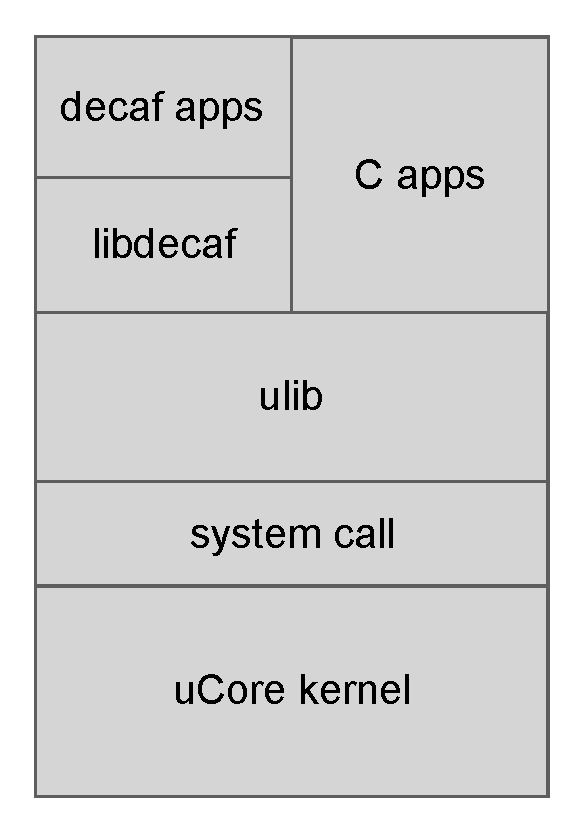
\includegraphics[width=0.3\linewidth]{decaf.pdf}
    \caption{Decaf标准库实现层次结构}
    \label{figure:libdecaf}
\end{figure}

Allocate在ulib中没有对应的实现。由于Decaf只分配内存而不释放,我们在libdecaf的中增加了一个静态数组作为Decaf程序的堆,调用Allocate时,首先将长度进行四字节对齐,然后返回数组相应元素的地址。

\subsection{与平台约定衔接}
Decaf 进行函数调用时,会将参数从右到左依次压入栈中,而在uCore系统中前四个参数分别保存在a0到a3寄存器中,其余参数压入栈中。因此,为了使得 Decaf 程序能够调用 C 编写的 libdecaf 中的函数,需对 Decaf 的标准库函数调用进行封装。我们使用汇编语言编写标准库函数调用的封装(\texttt{decafCall.S}),在调用时将参数从栈中取出,保存在对应的寄存器中,然后调用libdecaf的对应函数,以完成ABI的转换。以 \texttt{PrintString} 函数为例,核心代码如下所示。

\begin{minted}{asm}
    .type    __c_call, @function
__c_call:
    addiu   $sp, $sp, -20
    sw      $ra, 16($sp)
    la      $ra, __c_call_after_call
    jr      $t0

    __c_call_after_call:
    lw      $ra, 16($sp)
    addiu   $sp, $sp, 20
    jr      $ra


    .type   _PrintString, @function
_PrintString:
    lw      $a0, 4($sp)
    la      $t0, __decaf_printString
    j       __c_call
\end{minted}

uCore的用户态程序正常退出时应返回(在v0寄存器中保存)0,而Decaf程序的主函数没有返回值。为使其正确返回0,我们修改了 Decaf 编译器的后端,将Decaf程序主函数的名称修改为\texttt{\_\_decaf\_main}。同时,在 libdecaf 中加入main函数,调用\texttt{\_\_decaf\_main}并返回0。

我们将 Decaf 程序的编译加入了uCore系统的编译过程。在编译用户态程序时,首先检查\texttt{user}目录下是否存在Decaf源文件,若存在则调用编译原理课程提供的Decaf编译器将源文件编译为MIPS汇编,进而使用汇编器将其转换为目标文件,目标文件与 libdecaf 和 ulib 链接。uCore 中的用户态程序的入口为 ulib 中的 \texttt{umain} 函数,这一点通过在链接时指定链接脚本 \texttt{user/libs/user.ld} 完成。

\section{Linux操作系统}

Linux 是最为著名的开源操作系统,有丰富的软硬件支持。我们以 Linux 最新的稳定版本(v5.2.8)作为基线进行移植。

\subsection{CPU适配}

我们以 Linux 内核内置的 MIPS 4Kc CPU 为基础来实现移植,这是一款标准的 MIPS32 R1 CPU。首先我们需要添加 \texttt{TRIVIALMIPS} 这个架构,而后添加对应的架构目录(参见其他架构和 CPU 的目录结构即可)。

由于我们的 CPU 缺少一些功能(如 \texttt{Watch} 寄存器和 \texttt{PERF} 指令等),我们可以通过两种方式去除 Linux 的依赖。一方面,在 \texttt{arch/mips/include/asm/mach-trivialmips/} 目录下的 \texttt{cpu-features-overrides.h} 中可以通过定义类似 \texttt{cpu\_has\_watch} 的宏为 0,去除一些特定指令;另一方面,可以通过 \texttt{arch/mips/trivialmips/Platform} 文件来指定编译选项,如使用 \texttt{-mno-branch-likely} 去除 Branch Likely 等未实现的指令。

由于 NonTrivialMIPS 按照规范实现了 TLB 相关的 CP0 寄存器(包括 \texttt{Index, Wired, EntryHi, EntryLo, Random, PageMask} 等)与指令(包括 \texttt{TLBWI, TLBWR, TLBR} 等),因此无需修改 Linux 进程调度修改的代码。此外,Linux 也能够正常从 CP0 的 \texttt{Config1} 寄存器中得到 Cache 的相关属性(如大小、相连度)。对于浮点运算,当 Linux 检测到不存在 CP1 协处理器时,会自动使用软件模拟这些指令。因此,在 NonTrivialMIPS CPU 上运行 Linux 无需进行任何实际的指令简化工作。

\subsection{板级硬件适配}

除 CPU 适配之外,还需要在 Linux 内核代码树中进行下列的改动,以使得其能够在我们设计的 SoC 上工作:

\begin{description}
    \item[初始化代码] 这部分代码均位于 \texttt{arch/mips/trivialmips} 目录下,由多个 C 文件组成。需要完成的工作包括在引导早期阶段(即 \texttt{early\_printk} 使用的输出方式)初始化串口控制器并提供一个简单的输出函数(\texttt{prom\_putchar}),向内核注册 CPU 的中断控制器和时钟源,初始化设备树供后面的阶段使用。
    \item[设备树描述] 现代 Linux 使用设备树描述(Device Tree Description)来实现通用的驱动管理与配置,因此我们需要为开发板编写专门的设备树。所有的设备树都位于架构对应的 \texttt{boot/dts} 目录中,我们撰写了 \texttt{trivialmips/trivialmips\_nscscc.dts},其中描述了板载所有设备的信息,包括型号、寄存器地址分配、中断号与连接关系等。
    \item[默认内核配置] 内核默认配置保存在 \texttt{arch/mips/configs/} 目录中,我们提供了一个配置文件 \texttt{trivialmips\_nscscc\_defconfig},其中启用了实验板必须的驱动,以及调整了运行相关配置。
\end{description}

附录 \ref{sec:trivialmips-dts} 中包含了我们当前使用的 DTS 文件,其中描述了各个外设的信息供内核中的驱动程序进行匹配。

此外,我们还将 Linux 在默认图形终端(\texttt{tty1})上绘制的 Tux 企鹅 Logo 更换为清华大学校徽,以突出我们的移植工作。

\subsection{驱动移植}

Linux 中已经包含了相当多设备的驱动,只需要正确编写 DTS 文件提供信息即可使用。然而,有一些外设的驱动依旧需要移植或者修改。具体地,我们完成了下列的工作:

\begin{description}
    \item[USB控制器驱动] USB 控制器的驱动移植自 \texttt{ultra-embedded} 的开源代码,我们也进行了必要的修改以适应硬件的不同。驱动文件位于 \texttt{drivers/usb/host/ue11-hcd.c},能够将自己注册为 Linux 的标准 USB 2.0 Full Speed Host Controller。经过测试,该控制器驱动可以成功让 Linux 正确识别并操作挂接在 USB 3.0 Hub 下的 HID 设备和 Mass Storage 设备,能够使用键盘在图形终端进行输入、使 \texttt{xeyes} 程序响应鼠标事件,并可以挂载 U 盘上的存储分区并读取数据。
    \item[LCD控制器驱动] 板载的 NT35510 LCD 需要进行恰当的初始化以工作,每次写入数据时也需要先发送控制命令。我们从 \url{https://github.com/z4yx/linux-kernel} 处移植了一个可用的 NT35510 LCD 屏幕驱动,它会在 \texttt{/dev} 中创建名为 \texttt{nt35510} 的字符设备,只需向其写入 RGB565 格式的原始像素数据即可显示在屏幕上。同时,它还支持 \texttt{seek} 操作,可以修改屏幕的某个偏移处的像素数据,而无需全部刷新。
    \item[Framebuffer驱动] 内核自带的 \texttt{xilinxfb} 驱动能够正常使用,但是重绘等操作均使用内核自带的的 \texttt{cfb\_copyarea, cfg\_fillrect} 等函数,由 CPU 进行数据的拷贝,速度较慢。我们在驱动中重写了这些操作,调用我们在硬件中添加的 DMA 引擎(即 Framebuffer Reader 与 Writer)辅助完成这一工作,以提升控制台重绘的速度。 
    
\end{description}

完成驱动移植后,我们能够在 Framebuffer (VGA) 上绘制一个速度较快的图形终端,并使用 USB 键盘在终端中进行交互。同时,也能够在 LCD 屏幕上绘制任意的图象。

\subsection{用户态组件}

Linux 内核本身并不能提供任何用户态组件,因此我们需要手工编译这一部分。我们选择了著名的嵌入式 Linux 开发工具套件 \href{https://buildroot.org/}{Buildroot} 来协助完成用户程序的构建。构建过程中,我们选择了 \texttt{musl} 作为系统的 C/C++ 标准库实现,并使用 \texttt{busybox} 来提供大部分的命令行工具。

由于构建的 rootfs 较大,无法使用 initramfs 等方式直接加载,而 Flash 的读写速度也较慢并不灵活,因此我们使用 NFS 协议通过网络挂载系统的根分区。实践证明,在网络稳定的情况下,系统的响应速度并不会受到影响。

大部分 Linux 用户程序在我们的实验板上都可以正常运行,包括 GNU Coreutils、Python 解释器、网络工具(\texttt{ip, ping, mtr, wget, nc})等。由于我们实现了加速的 Framebuffer,因此 Xorg Server 能够正常初始化图形设备,运行 \texttt{xscreenserver, xeyes, xterm} 等经典的 \texttt{XWindow} 图形程序,并且它们都能正确处理来自 USB 键盘、鼠标的输入。同时,我们也能够基于 Qt 等现代化图形框架正常编写程序进行演示。

% \subsection{示例:Qt 图形程序}

% \todo

\subsection{示例:软硬件协同设计(AES加速)}

\texttt{OpenSSL} 是著名的开源密码学算法库。为了利用第 \ref{sec:enhancement} 节中提到的 CPU 内置的密码学加速单元,我们修改了 \texttt{OpenSSL 1.1.1c} 的源代码,采用我们编写的 C 代码替换原有的汇编实现。为了替换 AES 加密算法,共需要修改四个函数,其定义及功能见表 \ref{table:openssl} 所示。

\begin{table}[htbp]
    \centering
    \caption{OpenSSL AES 实现}
    \label{table:openssl}
\begin{tabular}{|l|l|}
\hline
名称 & 功能 \\ \hline
\texttt{AES\_set\_encrypt\_key} & 设置加密密钥,支持128位和256位两种密钥长度 \\ \hline
\texttt{AES\_encrypt} & 对 32 字节的块进行 AES 加密 \\ \hline
\texttt{AES\_set\_decrypt\_key} & 设置解密密钥,支持128位和256位两种密钥长度 \\ \hline
\texttt{AES\_decrypt} & 对 32 字节的块进行 AES 解密 \\ \hline
\end{tabular}
\end{table}

我们在代码中提供了这四个函数的实现,通过在 C 代码中内嵌汇编(见附录 \ref{sec:cp2-rw}) 向 AES 协处理器交换数据,包括写入密钥,设置密钥长度和模式,输入数据并读出数据,按照函数结构进行内存的读写。为了使得加速更加显著,由于加密算法默认采用大端序,而 CPU 运行在小端序,我们在 mfc2 指令中选择一个位指示由硬件进行端序翻转。最终测试结果如表 \ref{table:openssl-speedup} 所示,最大加速比可达 11 倍左右,提升显著。

\begin{table}[htbp]
    \centering
    \caption{OpenSSL AES(采用 \texttt{aes-128-cbc} 模式)加解密性能比较}
    \label{table:openssl-speedup}
\begin{tabular}{|c|c|c|}
\hline
块大小 & 原吞吐量 (MB/s) & 硬件加速后吞吐量(MB/s)\\ \hline
16 Bytes & 0.85 & 5.94 \\ \hline
64 Bytes & 0.97 & 8.91 \\ \hline
256 Bytes & 1.00 & 10.52 \\ \hline
1024 Bytes & 1.01 & 11.02 \\ \hline
8192 Bytes & 1.01 & 10.51 \\ \hline
\end{tabular}
\end{table}

由于 \texttt{OpenSSL} 提供的密码学算法库 \texttt{libcrypto} 被系统中的多个程序(如 \texttt{ssh, scp, wget})所使用,因此这一修改也能被应用到这些工具软件中,取得同样显著的性能提升。


\subsection{演示程序:TrivialDashboard}

为了充分利用 SoC 实现的功能和优化,我们使用 Qt5 图形框架编写了演示程序 TrivialDashboard,可以监控本机或者远程计算机上 CPU 和网络资源的利用率,可以响应用户的鼠标、键盘输入,并且内置一个虚拟终端。

远程连接通过 SSH 完成,我们选择了 \texttt{LibSSH} 作为协议支持库。\texttt{LibSSH} 可以选择链接到 OpenSSL 提供的 \texttt{libcrypto},从而利用 上一节中提到的 AES 硬件优化。在开启优化后可以看到显著的传输速率提升。

我们使用开源的 \texttt{qtermwidget} 项目提供虚拟终端组件,该组件支持鼠标选中、滚动、搜索和在程序内复制粘贴。

在渲染时,程序通过使用 Qt5 提供的 \texttt{linuxfb} 驱动,直接跳过 XWindow 和 Xorg Server,在 Framebuffer 层完成用户界面绘制,可以充分利用硬件 DMA 优化,在开启抗锯齿之后仍能达到较高的刷新率。

这一演示程序在 Windows 上开发,大量使用了 C++17 的特性,包括使用 \texttt{std::mutex} 和 \texttt{std::unique\_lock} 进行连接的同步操作。代码可以直接交叉编译之后在 SoC 上运行的 Linux 系统中正常工作。


\chapter{自动化测试}

为了保证实现的正确性,本项目进行了自动化的集成、测试与部署。所有的流程都通过Docker进行,确保是可完整复现的。

\section{硬件测试}
\label{section:test_hardware}

本项目使用的主要硬件设计语言SystemVerilog是一门强大的验证语言,我们用它编写testbench来测试硬件模块。主要的测试用例分为有:

\begin{description}
    \item[CPU测试] 本部分用于测试CPU实现指令的正确性。我们对CPU的各条指令都编写了相应的测试程序,同时还对各类可能的冲突现象、异常、TLB的行为编写了对应的测试。测试的过程是通过一个testbench虚拟出外部的总线和RAM并且接入CPU,并对CPU中的访存动作,包括WB阶段对寄存器和的写请求和MEM阶段的内存写请求进行监视。每个测试用例对上述动作都会给出响应期待的结果,同时在运行testbench时会将监测到的真实的写请求和期望的结果进行对比进而确认程序执行的正确性。整个CPU的测试过程是自动化的,通过指定格式的汇编代码即可生成对应的存储文件(\texttt{.mem}文件)、答案文件(\texttt{.ans}文件);我们编写了用于执行上述动作的 SystemVerilog task,可以直接使用 Vivado 对所有用例依次执行测试,得到比较结果,无需人工介入观察信号,如果发现真实的运行和期望不符会进行报告。所有的测试用例以及解释可见表\ref{table:cpu_testbenches}。除此之外,我们还在CPU仿真部分引入了Verilator这一基于C++的编译型仿真工具,用于简单的测试,其性能相比解释型工具有数量级上的增强。
    \item[Cache 测试] 我们生成不同特征的访存序列(顺序/随机),并捕获真实应用程序的访存序列,将其作为激励传递给 Cache 组件,观察其行为是否与预期一致,本部分用于测试 Cache 的正确性。此部分还使用了一个 AXI RAM 的行为模型,用于替代 Xilinx AXI Block RAM Generator IP 核,并能模拟测试中人工插入的延迟。

\end{description}

同时,我们还为龙芯功能测试、性能测试编写 tcl 脚本并修改 testbench,以在 CI 环境中能够进行自动化测试和结果提取。最后,还可以自动生成上述测试的 bitstream 文件,供直接上板测试。

对于主分支的每一次提交,都需要进行持续集成(CI),步骤包括进行IP核的生成与预综合、上述的测试,以及 bitstream 的生成。由于完整仿真速度较慢,通常只运行CPU测试部分。

\begin{table}[!htbp]
\centering
\caption{CPU测试用例(位于 \texttt{testbench/cpu/testcases} 目录中)}
\label{table:cpu_testbenches}
\begin{threeparttable}
\begin{tabular}{|l|l|}
\hline
\multicolumn{1}{|c|}{\textbf{文件名}} & \multicolumn{1}{c|}{\textbf{测试内容}}                                                                                        \\ \hline
except/*              & 异常相关测试          \\ \hline                           
instr/*              & 指令功能测试          \\ \hline                           
branch/*              & 分支测试          \\ \hline                              
hazard/*              & 各类边界情况测试          \\ \hline                      
across\_tlb/*              & TLB测试          \\ \hline                          
performance/*              & 性能测试          \\ \hline                                   \end{tabular}
\end{threeparttable}
\end{table}

\section{软件测试}

在软件方面,本项目计划对编写的所有汇编/C/C++代码,移植的Bootloader、操作系统,以及需要运行的功能测试、性能测试,均编写基于GitLab CI的持续集成脚本,保证每个版本都能进行正确的、可重现的编译。

\addcontentsline{toc}{chapter}{\listfigurename}

\listoffigures

\addcontentsline{toc}{chapter}{\listtablename}

\listoftables

\appendix

\chapter{声明与致谢}

\section{版权声明}

本项目涉及的代码均在 GitHub 开放,相应的仓库列举如下(名称即为链接):

\begin{description}
    \item[\href{https://github.com/trivialmips/TrivialMIPS}{\color{blue} TrivialMIPS}] 初版的 CPU 设计(运行在清华大学 ThinPad 实验板上)
    \item[\href{https://github.com/trivialmips/nontrivial-mips}{\color{blue} NonTrivialMIPS}] 最终提交的 CPU 设计(运行在龙芯实验板上)
    \item[\href{https://github.com/trivialmips/TrivialMIPS_Software}{\color{blue} Software}] C++ 编写的裸机(Baremetal)程序,包括 TrivialBootloader 等
    \item[\href{https://github.com/trivialmips/u-boot-trivialmips}{\color{blue} U-Boot}] 移植的 U-Boot 引导程序
    \item[\href{https://github.com/trivialmips/u-boot-trivialmips}{\color{blue} uCore}] 移植的 uCore 操作系统
    \item[\href{https://github.com/trivialmips/linux-nontrivial-mips}{\color{blue} Linux}] 移植的 Linux 内核
    \item[\href{https://github.com/trivialmips/openssl}{\color{blue} OpenSSL}] 适配硬件 AES 加速功能的 OpenSSL 程序
    \item[\href{https://github.com/trivialmips/trivial-dashboard}{\color{blue} TrivialDashboard}] 使用 Qt 撰写的 Dashboard 演示程序
\end{description}

这些项目均遵循它们特定的开源许可证,某些目录中可能包含受版权保护的内容,使用它们意味着您知晓并愿意承担任何可能的法律责任。

本报告著作权归作者所有。您被允许在不作任何修改的情况下重新分发此文档;未经许可,您不得以任何方式复制、引用或演绎其中的任何内容。

\section{致谢}

本项目开发过程中得到了来自清华大学计算机系张宇翔同学的大力支持,我们在此表示衷心的感谢。此外,我们的指导教师陈康老师、刘卫东老师给我们提出了许多宝贵的建议,唐适之同学、王邈同学、刘家昌同学也向我们提供了帮助,在此一并向他们表示感谢。

\chapter{代码摘录}

\section{TrivialBootloader 使用的链接脚本}
\label{sec:linker-script}

\begin{minted}{c}
ENTRY(_start);

MEMORY
{
    BOOTROM  (rx)  : ORIGIN = 0xBFC00000, LENGTH = 128K
    OCM      (rwx) : ORIGIN = 0x88000000, LENGTH = 64K
    RAM      (rwx) : ORIGIN = 0x80000000, LENGTH = 128M
}

#ifdef CODE_INTO_BOOTROM
#define TEXT_AREA BOOTROM
#define DATA_AREA OCM
#else
#define TEXT_AREA OCM
#define DATA_AREA RAM
#endif

SECTIONS
{
    . = ORIGIN(TEXT_AREA);

    _mem_start = ORIGIN(DATA_AREA);
    _mem_end = ORIGIN(DATA_AREA) + LENGTH(DATA_AREA);

#ifdef CODE_INTO_BOOTROM
    _mem_avail_start = ORIGIN(RAM);
    _mem_avail_end = ORIGIN(RAM) + LENGTH(RAM);
#else
    _mem_avail_start = _stack;
    _mem_avail_end = ORIGIN(RAM) + LENGTH(RAM);
#endif

    .text :
    {
        _text = .;
        *(.text.startup)
        *(.text*)
        *(.rodata*)
        *(.reginfo)
        *(.init)
        *(.stub)
        *(.gnu.warning)
        *(.MIPS.abiflags)
        _text_end = .;
    } > TEXT_AREA

    .data :
    {
        _data = .;
        _stack = _data + LENGTH(DATA_AREA) - 32;
        *(.data)
        *(.data*)
        *(.eh_frame)
        _gp = ALIGN(16);  
        *(.got.plt) *(.got)
        *(.sdata) 
        *(.lit8) 
        *(.lit4)
        _data_end = .;
    } > DATA_AREA

    .sbss : 
    { 
        *(.sbss)
        *(.scommon)
    } > DATA_AREA
    
    .bss :
    {
        _bss = .;
        *(.dynbss)
        *(.bss)
        *(COMMON)
        _bss_end = .;
    } > DATA_AREA

    /DISCARD/ :
    {
        *(.note*);
        *(.iplt*);
        *(.igot*);
        *(.rel*);
        *(.comment);
    }
}
\end{minted}

\section{扩展计算单元的寄存器读写}
\label{sec:cp2-rw}
\begin{minted}{c++}
#define write_aes_register_bigendian(addr, variable)       \
  asm volatile(".byte " #addr "\n"                        \
               ".byte 0x81\n"                             \
               ".byte 0b10000000+(%0-0x100)\n"            \
               ".byte 0b01001000\n"                       \
               :                                          \
               : "r"(variable));

#define read_aes_register_bigendian(addr, variable)       \
  asm volatile(".byte " #addr "\n"                        \
               ".byte 0x81\n"                             \
               ".byte 0b00000000+(%0-0x100)\n"            \
               ".byte 0b01001000\n"                       \
               : "=r"(variable));

#define write_aes_register(addr, variable)                \
  asm volatile(".byte " #addr "\n"                        \
               ".byte 0x01\n"                             \
               ".byte 0b10000000+(%0-0x100)\n"            \
               ".byte 0b01001000\n"                       \
               :                                          \
               : "r"(variable));

#define read_aes_register(addr, variable)                 \
  asm volatile(".byte " #addr "\n"                        \
               ".byte 0x01\n"                             \
               ".byte 0b00000000+(%0-0x100)\n"            \
               ".byte 0b01001000\n"                       \
               : "=r"(variable));
\end{minted}

\section{移植 Linux 使用的 DTS文件}
\label{sec:trivialmips-dts}

\begin{minted}{text}
/dts-v1/;

#include <dt-bindings/interrupt-controller/irq.h>

/ {
    compatible = "TrivialMIPS,NSCSCC";
    #address-cells = <1>;
    #size-cells = <1>;

    chosen {
        bootargs = "console=ttyS0,115200n8 console=tty1 rootfstype=squashfs root=/dev/mtdblock1";
    };

    aliases {
            serial0 = &serial0;
        };

    cpus {
        #address-cells = <1>;
        #size-cells = <0>;
        cpu@0 {
            device_type = "cpu";
            compatible = "mips,4Kc";
            clocks = <&ext>;
            reg = <0>;
        };
    };

    ext: ext {
        compatible = "fixed-clock";
        clock-frequency = <80000000>;
        #clock-cells = <0>;
    };

    memory {
        device_type = "memory";
        reg = <0x0 0x8000000>;
    };

    cpuintc: interrupt-controller@0 {
        #address-cells = <0>;
        #interrupt-cells = <1>;
        interrupt-controller;
        compatible = "mti,cpu-interrupt-controller";
    };

    soc {
        compatible = "simple-bus";
        #address-cells = <1>;
        #size-cells = <1>;
        #interrupt-cells = <1>;
        ranges;

        serial0: serial@1fd02000 {
            device_type = "serial";
            compatible = "ns16550a";
            reg = <0x1fd02000 0x1000>;
            reg-offset = <0x1000>;
            reg-io-width = <4>;
            reg-shift = <2>;
            current-speed = <115200>;
            clock-frequency = <100000000>;
            interrupt-parent = <&cpuintc>;
            interrupts = <2>;
        };

        lcd0: lcd@1c030000 {
            compatible = "lcd,nt35510";
            reg = <0x1c030000 0x1000>;
        };

        axi_quad_spi: spi@1c040000 {
            #address-cells = <1>;
            #size-cells = <0>;
            compatible = "xlnx,xps-spi-2.00.a";
            interrupt-parent = <&axi_intc_0>;
            interrupts = <1>;
            reg = <0x1c040000 0x10000>;
            xlnx,num-ss-bits = <0x1>;
            num-cs = <0x1>;
            fifo-size = <256>;

            flash@0 {
                compatible = "mx25l25635f", "jedec,spi-nor";
                reg = <0x0>;
                spi-max-frequency = <30000000>;

                spi-rx-bus-width = <4>;
                m25p,fast-read;

                partitions {
                    compatible = "fixed-partitions";
                    #address-cells = <1>;
                    #size-cells = <1>;

                    partition@10000 {
                        label = "bootenv";
                        reg = <0x10000 0x10000>;
                    };
                    partition@20000 {
                        label = "rootfs";
                        reg = <0x20000 0x1fe0000>;
                    };
                };
            };
        };

        axi_intc_0: interrupt-controller@1d000000 {
            #interrupt-cells = <1>;
            compatible = "xlnx,xps-intc-1.00.a";
            interrupt-controller;
            interrupt-parent = <&cpuintc>;
            interrupts = <6>;
            reg = <0x1d000000 0x1000>;
            xlnx,kind-of-intr = <0x15>;
            xlnx,num-intr-inputs = <0x4>;
        };

        axi_ethernetlite: ethernet@1c000000 {
            compatible = "xlnx,xps-ethernetlite-3.00.a";
            device_type = "network";
            mac-address = [19 98 00 01 00 29];
            phy-handle = <&phy0>;
            reg = <0x1c000000 0x10000>;
            xlnx,duplex = <0x1>;
            xlnx,include-global-buffers = <0x1>;
            xlnx,include-internal-loopback = <0x0>;
            xlnx,include-mdio = <0x1>;
            xlnx,instance = "axi_ethernetlite_inst";
            xlnx,rx-ping-pong = <0x1>;
            xlnx,s-axi-id-width = <0x1>;
            xlnx,tx-ping-pong = <0x1>;
            xlnx,use-internal = <0x0>;
            interrupt-parent = <&axi_intc_0>;
            interrupts = <0>;
            mdio {
                #address-cells = <1>;
                #size-cells = <0>;
                phy0: phy@1 {
                    device_type = "ethernet-phy";
                    reg = <1>;
                } ;
            } ;
        } ;

        ps2: ps2@1c020000 {
            compatible = "altr,ps2-1.0";
            reg = <0x1c020000 0x1000>;
            interrupt-parent = <&cpuintc>;
            interrupts = <3>;
        };

        usb: usb@1c050000 {
            compatible = "ue11-hcd";
            reg = <0x1c050000 0x1000>;
            interrupt-parent = <&axi_intc_0>;
            interrupts = <3>;
        };

        axi_tft_0: axi_tft@1c010000 {
            compatible = "xlnx,xps-tft-1.00.accl";
            reg = <0x1c010000 0x1000>, // TFT controller
                <0x1c060000 0x1000>, // framebuffer read
                <0x1c070000 0x1000>, // framebuffer write
                <0x1ff08000 0x4>; // video stream modifier control
            xlnx,dcr-splb-slave-if = <0x1>;
            resolution = <640 480>; // actual video size
            virtual-resolution = <1024 480>; // framebuffersize
            phys-size = <640 480>; // don't care (physical size of screen)
        };

    };
};
\end{minted}

\end{document}
